\documentclass[twoside]{book}

% Packages required by doxygen
\usepackage{fixltx2e}
\usepackage{calc}
\usepackage{doxygen}
\usepackage[export]{adjustbox} % also loads graphicx
\usepackage{graphicx}
\usepackage[utf8]{inputenc}
\usepackage{makeidx}
\usepackage{multicol}
\usepackage{multirow}
\PassOptionsToPackage{warn}{textcomp}
\usepackage{textcomp}
\usepackage[nointegrals]{wasysym}
\usepackage[table]{xcolor}

% Font selection
\usepackage[T1]{fontenc}
\usepackage[scaled=.90]{helvet}
\usepackage{courier}
\usepackage{amssymb}
\usepackage{sectsty}
\renewcommand{\familydefault}{\sfdefault}
\allsectionsfont{%
  \fontseries{bc}\selectfont%
  \color{darkgray}%
}
\renewcommand{\DoxyLabelFont}{%
  \fontseries{bc}\selectfont%
  \color{darkgray}%
}
\newcommand{\+}{\discretionary{\mbox{\scriptsize$\hookleftarrow$}}{}{}}

% Page & text layout
\usepackage{geometry}
\geometry{%
  a4paper,%
  top=2.5cm,%
  bottom=2.5cm,%
  left=2.5cm,%
  right=2.5cm%
}
\tolerance=750
\hfuzz=15pt
\hbadness=750
\setlength{\emergencystretch}{15pt}
\setlength{\parindent}{0cm}
\setlength{\parskip}{3ex plus 2ex minus 2ex}
\makeatletter
\renewcommand{\paragraph}{%
  \@startsection{paragraph}{4}{0ex}{-1.0ex}{1.0ex}{%
    \normalfont\normalsize\bfseries\SS@parafont%
  }%
}
\renewcommand{\subparagraph}{%
  \@startsection{subparagraph}{5}{0ex}{-1.0ex}{1.0ex}{%
    \normalfont\normalsize\bfseries\SS@subparafont%
  }%
}
\makeatother

% Headers & footers
\usepackage{fancyhdr}
\pagestyle{fancyplain}
\fancyhead[LE]{\fancyplain{}{\bfseries\thepage}}
\fancyhead[CE]{\fancyplain{}{}}
\fancyhead[RE]{\fancyplain{}{\bfseries\leftmark}}
\fancyhead[LO]{\fancyplain{}{\bfseries\rightmark}}
\fancyhead[CO]{\fancyplain{}{}}
\fancyhead[RO]{\fancyplain{}{\bfseries\thepage}}
\fancyfoot[LE]{\fancyplain{}{}}
\fancyfoot[CE]{\fancyplain{}{}}
\fancyfoot[RE]{\fancyplain{}{\bfseries\scriptsize Generated by Doxygen }}
\fancyfoot[LO]{\fancyplain{}{\bfseries\scriptsize Generated by Doxygen }}
\fancyfoot[CO]{\fancyplain{}{}}
\fancyfoot[RO]{\fancyplain{}{}}
\renewcommand{\footrulewidth}{0.4pt}
\renewcommand{\chaptermark}[1]{%
  \markboth{#1}{}%
}
\renewcommand{\sectionmark}[1]{%
  \markright{\thesection\ #1}%
}

% Indices & bibliography
\usepackage{natbib}
\usepackage[titles]{tocloft}
\setcounter{tocdepth}{3}
\setcounter{secnumdepth}{5}
\makeindex

% Hyperlinks (required, but should be loaded last)
\usepackage{ifpdf}
\ifpdf
  \usepackage[pdftex,pagebackref=true]{hyperref}
\else
  \usepackage[ps2pdf,pagebackref=true]{hyperref}
\fi
\hypersetup{%
  colorlinks=true,%
  linkcolor=blue,%
  citecolor=blue,%
  unicode%
}

% Custom commands
\newcommand{\clearemptydoublepage}{%
  \newpage{\pagestyle{empty}\cleardoublepage}%
}

\usepackage{caption}
\captionsetup{labelsep=space,justification=centering,font={bf},singlelinecheck=off,skip=4pt,position=top}

%===== C O N T E N T S =====

\begin{document}

% Titlepage & ToC
\hypersetup{pageanchor=false,
             bookmarksnumbered=true,
             pdfencoding=unicode
            }
\pagenumbering{alph}
\begin{titlepage}
\vspace*{7cm}
\begin{center}%
{\Large Vid\+Chaser \\[1ex]\large 2.\+4.\+20170727 }\\
\vspace*{1cm}
{\large Generated by Doxygen 1.8.13}\\
\end{center}
\end{titlepage}
\clearemptydoublepage
\pagenumbering{roman}
\tableofcontents
\clearemptydoublepage
\pagenumbering{arabic}
\hypersetup{pageanchor=true}

%--- Begin generated contents ---
\chapter{Namespace Index}
\section{Namespace List}
Here is a list of all namespaces with brief descriptions\+:\begin{DoxyCompactList}
\item\contentsline{section}{\hyperlink{namespace_vid_chaser}{Vid\+Chaser} }{\pageref{namespace_vid_chaser}}{}
\end{DoxyCompactList}

\chapter{Class Index}
\section{Class List}
Here are the classes, structs, unions and interfaces with brief descriptions\+:\begin{DoxyCompactList}
\item\contentsline{section}{\hyperlink{class_matrix_util}{Matrix\+Util} }{\pageref{class_matrix_util}}{}
\item\contentsline{section}{\hyperlink{class_shader_util}{Shader\+Util} }{\pageref{class_shader_util}}{}
\end{DoxyCompactList}

\chapter{File Index}
\section{File List}
Here is a list of all files with brief descriptions\+:\begin{DoxyCompactList}
\item\contentsline{section}{C\+:/\+Workspace/\+Vid\+Chaser/\+Platform/\+Vid\+Chaser\+Android/\+Vid\+Chaser/src/main/java/com/maxst/vidchaser/\hyperlink{_camera1_controller_8java}{Camera1\+Controller.\+java} }{\pageref{_camera1_controller_8java}}{}
\item\contentsline{section}{C\+:/\+Workspace/\+Vid\+Chaser/\+Platform/\+Vid\+Chaser\+Android/\+Vid\+Chaser/src/main/java/com/maxst/vidchaser/\hyperlink{_camera2_controller_8java}{Camera2\+Controller.\+java} }{\pageref{_camera2_controller_8java}}{}
\item\contentsline{section}{C\+:/\+Workspace/\+Vid\+Chaser/\+Platform/\+Vid\+Chaser\+Android/\+Vid\+Chaser/src/main/java/com/maxst/vidchaser/\hyperlink{_camera_controller_8java}{Camera\+Controller.\+java} }{\pageref{_camera_controller_8java}}{}
\item\contentsline{section}{C\+:/\+Workspace/\+Vid\+Chaser/\+Platform/\+Vid\+Chaser\+Android/\+Vid\+Chaser/src/main/java/com/maxst/vidchaser/\hyperlink{_camera_size_8java}{Camera\+Size.\+java} }{\pageref{_camera_size_8java}}{}
\item\contentsline{section}{C\+:/\+Workspace/\+Vid\+Chaser/\+Platform/\+Vid\+Chaser\+Android/\+Vid\+Chaser/src/main/java/com/maxst/vidchaser/\hyperlink{_camera_surface_view_8java}{Camera\+Surface\+View.\+java} }{\pageref{_camera_surface_view_8java}}{}
\item\contentsline{section}{C\+:/\+Workspace/\+Vid\+Chaser/\+Platform/\+Vid\+Chaser\+Android/\+Vid\+Chaser/src/main/java/com/maxst/vidchaser/\hyperlink{_on_new_camera_frame_callback_8java}{On\+New\+Camera\+Frame\+Callback.\+java} }{\pageref{_on_new_camera_frame_callback_8java}}{}
\item\contentsline{section}{C\+:/\+Workspace/\+Vid\+Chaser/\+Platform/\+Vid\+Chaser\+Android/\+Vid\+Chaser/src/main/java/com/maxst/vidchaser/\hyperlink{_projection_matrix_8java}{Projection\+Matrix.\+java} }{\pageref{_projection_matrix_8java}}{}
\item\contentsline{section}{C\+:/\+Workspace/\+Vid\+Chaser/\+Platform/\+Vid\+Chaser\+Android/\+Vid\+Chaser/src/main/java/com/maxst/vidchaser/\hyperlink{_surface_manager_8java}{Surface\+Manager.\+java} }{\pageref{_surface_manager_8java}}{}
\item\contentsline{section}{C\+:/\+Workspace/\+Vid\+Chaser/\+Platform/\+Vid\+Chaser\+Android/\+Vid\+Chaser/src/main/java/com/maxst/vidchaser/\hyperlink{_vid_chaser_a_p_i_8java}{Vid\+Chaser\+A\+P\+I.\+java} }{\pageref{_vid_chaser_a_p_i_8java}}{}
\item\contentsline{section}{C\+:/\+Workspace/\+Vid\+Chaser/\+Platform/\+Vid\+Chaser\+Android/\+Vid\+Chaser/src/main/java/com/maxst/vidchaser/\hyperlink{_vid_chaser_j_n_i_8java}{Vid\+Chaser\+J\+N\+I.\+java} }{\pageref{_vid_chaser_j_n_i_8java}}{}
\end{DoxyCompactList}

\chapter{Namespace Documentation}
\hypertarget{namespace_vid_chaser}{}\section{Vid\+Chaser Namespace Reference}
\label{namespace_vid_chaser}\index{Vid\+Chaser@{Vid\+Chaser}}
\subsection*{Enumerations}
\begin{DoxyCompactItemize}
\item 
enum \hyperlink{namespace_vid_chaser_a9a65fd4518380d53654f1af799cbf8ed}{Result\+Code} \{ \newline
\hyperlink{namespace_vid_chaser_a9a65fd4518380d53654f1af799cbf8eda5151e057ede3a1e7f376efbb56a0443e}{S\+U\+C\+C\+E\+SS} = 0, 
\hyperlink{namespace_vid_chaser_a9a65fd4518380d53654f1af799cbf8edab0d9537c24158b7ab8d23234c0808821}{F\+A\+IL} = 1, 
\hyperlink{namespace_vid_chaser_a9a65fd4518380d53654f1af799cbf8eda812155acd5fe876119863a7f884e7f4c}{M\+E\+M\+O\+R\+Y\+\_\+\+A\+L\+L\+O\+C\+A\+T\+I\+O\+N\+\_\+\+E\+R\+R\+OR} = 2, 
\hyperlink{namespace_vid_chaser_a9a65fd4518380d53654f1af799cbf8eda4d52f2f8000574e95b1ebc3dedc91298}{I\+N\+V\+A\+L\+I\+D\+\_\+\+A\+PP} = 10, 
\newline
\hyperlink{namespace_vid_chaser_a9a65fd4518380d53654f1af799cbf8edafd918f3fa6f9e5df38c8b0970dc0e51d}{T\+R\+A\+C\+K\+A\+B\+L\+E\+\_\+\+A\+L\+R\+E\+A\+D\+Y\+\_\+\+E\+X\+I\+ST} = 50, 
\hyperlink{namespace_vid_chaser_a9a65fd4518380d53654f1af799cbf8eda75a688e24ca224d5b9fe2859ea579f9c}{T\+R\+A\+C\+K\+A\+B\+L\+E\+\_\+\+I\+S\+\_\+\+N\+O\+T\+\_\+\+E\+X\+I\+ST} = 51, 
\hyperlink{namespace_vid_chaser_a9a65fd4518380d53654f1af799cbf8edafb2e81caca6ee6d10e83fb4a28921e39}{T\+R\+A\+C\+K\+A\+B\+L\+E\+\_\+\+A\+L\+R\+E\+A\+D\+Y\+\_\+\+A\+C\+T\+I\+V\+A\+T\+ED} = 52, 
\hyperlink{namespace_vid_chaser_a9a65fd4518380d53654f1af799cbf8eda2e2c5512767b66864b4db78ca8ab96ee}{T\+R\+A\+C\+K\+A\+B\+L\+E\+\_\+\+A\+L\+R\+E\+A\+D\+Y\+\_\+\+D\+E\+A\+C\+T\+I\+V\+A\+T\+ED} = 53, 
\newline
\hyperlink{namespace_vid_chaser_a9a65fd4518380d53654f1af799cbf8edac4e8d2fb08c509ce905b7821d8a028f1}{P\+I\+X\+E\+L\+\_\+\+F\+O\+R\+M\+A\+T\+\_\+\+E\+R\+R\+OR} = 60, 
\hyperlink{namespace_vid_chaser_a9a65fd4518380d53654f1af799cbf8edae75f339feb7a945186fcb40fc53280de}{I\+N\+P\+U\+T\+\_\+\+I\+M\+A\+G\+E\+\_\+\+E\+M\+P\+TY} = 61, 
\hyperlink{namespace_vid_chaser_a9a65fd4518380d53654f1af799cbf8eda40bd178f65d935a585199e4d178ebfe8}{I\+N\+P\+U\+T\+\_\+\+I\+M\+A\+G\+E\+\_\+\+R\+E\+S\+O\+L\+U\+T\+I\+O\+N\+\_\+\+E\+R\+R\+OR} = 62, 
\hyperlink{namespace_vid_chaser_a9a65fd4518380d53654f1af799cbf8edaf3c881f67a4378bb3039de82238456a5}{E\+N\+G\+I\+N\+E\+\_\+\+A\+L\+R\+E\+A\+D\+Y\+\_\+\+I\+N\+I\+T\+I\+A\+L\+I\+Z\+ED} = 170, 
\newline
\hyperlink{namespace_vid_chaser_a9a65fd4518380d53654f1af799cbf8edae356f1e1773cea2be2c7923c81c50b4d}{E\+N\+G\+I\+N\+E\+\_\+\+I\+S\+\_\+\+N\+O\+T\+\_\+\+I\+N\+I\+T\+I\+A\+L\+I\+Z\+ED} = 180, 
\hyperlink{namespace_vid_chaser_a9a65fd4518380d53654f1af799cbf8edae0af694ebbabbe2f9050b879bbab1650}{C\+H\+E\+C\+K\+\_\+\+L\+E\+A\+R\+N\+A\+B\+L\+E\+\_\+\+P\+I\+X\+E\+L\+F\+O\+R\+M\+A\+T\+\_\+\+E\+R\+R\+OR} = 190, 
\hyperlink{namespace_vid_chaser_a9a65fd4518380d53654f1af799cbf8edaf019ce4b932c9d8e30fcd49359e3bf2c}{L\+E\+A\+R\+N\+\_\+\+S\+T\+R\+O\+K\+E\+\_\+\+E\+M\+P\+TY} = 200, 
\hyperlink{namespace_vid_chaser_a9a65fd4518380d53654f1af799cbf8eda01e3cca957ead1e93450e8dbd49dc3b5}{L\+E\+A\+R\+N\+\_\+\+S\+T\+R\+O\+K\+E\+\_\+\+O\+V\+E\+R\+F\+L\+OW} = 201, 
\newline
\hyperlink{namespace_vid_chaser_a9a65fd4518380d53654f1af799cbf8eda3c8a1d9afcff42b2226ef6398019968d}{T\+R\+A\+C\+K\+E\+R\+\_\+\+A\+L\+R\+E\+A\+D\+Y\+\_\+\+S\+T\+A\+R\+T\+ED} = 300, 
\hyperlink{namespace_vid_chaser_a9a65fd4518380d53654f1af799cbf8eda0f6a6c38af8fed9e2315c7ca598470c9}{T\+R\+A\+C\+K\+E\+R\+\_\+\+A\+L\+R\+E\+A\+D\+Y\+\_\+\+S\+T\+O\+P\+ED} = 310, 
\hyperlink{namespace_vid_chaser_a9a65fd4518380d53654f1af799cbf8eda5c335d57b3c769c7eb00213f69d13b0b}{I\+N\+P\+U\+T\+\_\+\+T\+R\+A\+C\+K\+A\+B\+L\+E\+\_\+\+E\+M\+P\+TY} = 320, 
\hyperlink{namespace_vid_chaser_a9a65fd4518380d53654f1af799cbf8eda1099645fafffff33a4e4db2aab5abb4d}{U\+N\+D\+E\+F\+I\+N\+E\+\_\+\+E\+R\+R\+OR} = 99
 \}
\end{DoxyCompactItemize}
\subsection*{Functions}
\begin{DoxyCompactItemize}
\item 
\hyperlink{_vid_chaser_a_p_i_8h_abe868bb94e22f611aece5087695f9ef3}{V\+I\+D\+C\+H\+A\+S\+E\+R\+\_\+\+A\+PI} char $\ast$ \hyperlink{namespace_vid_chaser_a351a56150e8d7cb4a2eb78a5332f6efc}{get\+Engine\+Version} ()
\begin{DoxyCompactList}\small\item\em get engine version. \end{DoxyCompactList}\item 
\hyperlink{_vid_chaser_a_p_i_8h_abe868bb94e22f611aece5087695f9ef3}{V\+I\+D\+C\+H\+A\+S\+E\+R\+\_\+\+A\+PI} void \hyperlink{namespace_vid_chaser_a9382813c29f7bf8b97fdc9f6e2e9b51d}{start\+Camera} (int camera\+Id, int width, int height, std\+::string extra=std\+::string())
\begin{DoxyCompactList}\small\item\em start a \#camera\+Id camera with width and height resolution \end{DoxyCompactList}\item 
\hyperlink{_vid_chaser_a_p_i_8h_abe868bb94e22f611aece5087695f9ef3}{V\+I\+D\+C\+H\+A\+S\+E\+R\+\_\+\+A\+PI} void \hyperlink{namespace_vid_chaser_ad7ef05eaf00e73b7f35f760e59c5ecca}{stop\+Camera} ()
\begin{DoxyCompactList}\small\item\em close the operating camera \end{DoxyCompactList}\item 
\hyperlink{_vid_chaser_a_p_i_8h_abe868bb94e22f611aece5087695f9ef3}{V\+I\+D\+C\+H\+A\+S\+E\+R\+\_\+\+A\+PI} void \hyperlink{namespace_vid_chaser_acb17083d4c7121491e9563358d3e018f}{set\+Preview\+Callback} (Camera\+Preview\+Callback callback)
\begin{DoxyCompactList}\small\item\em register callback using camera preview buffer \end{DoxyCompactList}\item 
\hyperlink{_vid_chaser_a_p_i_8h_abe868bb94e22f611aece5087695f9ef3}{V\+I\+D\+C\+H\+A\+S\+E\+R\+\_\+\+A\+PI} void \hyperlink{namespace_vid_chaser_a563757135fd48e2a0c9b14349271c6ac}{init\+Rendering} ()
\begin{DoxyCompactList}\small\item\em initialize an internal resource for rendering \end{DoxyCompactList}\item 
\hyperlink{_vid_chaser_a_p_i_8h_abe868bb94e22f611aece5087695f9ef3}{V\+I\+D\+C\+H\+A\+S\+E\+R\+\_\+\+A\+PI} void \hyperlink{namespace_vid_chaser_afbfe1bf77862004fd5da9c95194cc506}{update\+Rendering} (int screen\+Width, int screen\+Height)
\begin{DoxyCompactList}\small\item\em input information necessary for calculating projection matrix \end{DoxyCompactList}\item 
\hyperlink{_vid_chaser_a_p_i_8h_abe868bb94e22f611aece5087695f9ef3}{V\+I\+D\+C\+H\+A\+S\+E\+R\+\_\+\+A\+PI} void \hyperlink{namespace_vid_chaser_a76a9d325e6621b9c163c5154db3f3141}{set\+Screen\+Orientation} (\hyperlink{_vid_chaser_define_8h_a5af96ebe9fdc47f01c3989cf97d41a77}{Screen\+Orientation} orientation)
\begin{DoxyCompactList}\small\item\em set Screen Orientation \end{DoxyCompactList}\item 
\hyperlink{_vid_chaser_a_p_i_8h_abe868bb94e22f611aece5087695f9ef3}{V\+I\+D\+C\+H\+A\+S\+E\+R\+\_\+\+A\+PI} void \hyperlink{namespace_vid_chaser_a68f76b454b274f9be3486792dbfd93a5}{render\+Scene} ()
\begin{DoxyCompactList}\small\item\em draw background Image. \end{DoxyCompactList}\item 
\hyperlink{_vid_chaser_a_p_i_8h_abe868bb94e22f611aece5087695f9ef3}{V\+I\+D\+C\+H\+A\+S\+E\+R\+\_\+\+A\+PI} void \hyperlink{namespace_vid_chaser_a5efdacefec8542b2d3935b87303dd442}{deinit\+Rendering} ()
\begin{DoxyCompactList}\small\item\em deinitialize an internal resource for rendering \end{DoxyCompactList}\item 
\hyperlink{_vid_chaser_a_p_i_8h_abe868bb94e22f611aece5087695f9ef3}{V\+I\+D\+C\+H\+A\+S\+E\+R\+\_\+\+A\+PI} \hyperlink{namespace_vid_chaser_a9a65fd4518380d53654f1af799cbf8ed}{Result\+Code} \hyperlink{namespace_vid_chaser_ac6f30324b16909dc9916e2e80326ada4}{create} (std\+::string app\+Signature=\char`\"{}For\+\_\+\+Mobile\char`\"{})
\begin{DoxyCompactList}\small\item\em create Engine. \end{DoxyCompactList}\item 
\hyperlink{_vid_chaser_a_p_i_8h_abe868bb94e22f611aece5087695f9ef3}{V\+I\+D\+C\+H\+A\+S\+E\+R\+\_\+\+A\+PI} \hyperlink{namespace_vid_chaser_a9a65fd4518380d53654f1af799cbf8ed}{Result\+Code} \hyperlink{namespace_vid_chaser_a3ef5c1fa7f048b2a32cd1d7b2dde1cd4}{add\+Tracking\+Point} (int x, int y, int $\ast$idx, \hyperlink{_vid_chaser_define_8h_ab7550d874bc06c5d36e27af27c7381e9}{Tracking\+Method} tracking\+Method=\hyperlink{_vid_chaser_define_8h_ab7550d874bc06c5d36e27af27c7381e9aecccd1296dcfe0ddcbe5954f37899f19}{Tracking\+Method\+::\+T\+R\+A\+N\+S\+L\+A\+T\+I\+ON})
\begin{DoxyCompactList}\small\item\em Add tracking position(image coordinate). \end{DoxyCompactList}\item 
\hyperlink{_vid_chaser_a_p_i_8h_abe868bb94e22f611aece5087695f9ef3}{V\+I\+D\+C\+H\+A\+S\+E\+R\+\_\+\+A\+PI} \hyperlink{namespace_vid_chaser_a9a65fd4518380d53654f1af799cbf8ed}{Result\+Code} \hyperlink{namespace_vid_chaser_a80f0b4139cf0864085a72a5808fa6ce3}{activate\+Tracking\+Point} (int x, int y, int idx)
\begin{DoxyCompactList}\small\item\em activate tracking point \end{DoxyCompactList}\item 
\hyperlink{_vid_chaser_a_p_i_8h_abe868bb94e22f611aece5087695f9ef3}{V\+I\+D\+C\+H\+A\+S\+E\+R\+\_\+\+A\+PI} \hyperlink{namespace_vid_chaser_a9a65fd4518380d53654f1af799cbf8ed}{Result\+Code} \hyperlink{namespace_vid_chaser_aa9d6db3ede935229cbb4322665466192}{deactivate\+Tracking\+Point} (int idx)
\begin{DoxyCompactList}\small\item\em deactivate tracking point \end{DoxyCompactList}\item 
\hyperlink{_vid_chaser_a_p_i_8h_abe868bb94e22f611aece5087695f9ef3}{V\+I\+D\+C\+H\+A\+S\+E\+R\+\_\+\+A\+PI} \hyperlink{namespace_vid_chaser_a9a65fd4518380d53654f1af799cbf8ed}{Result\+Code} \hyperlink{namespace_vid_chaser_a3926d98471a7a7f01c2537121b27dd35}{remove\+Tracking\+Point} (int idx)
\begin{DoxyCompactList}\small\item\em Remove the tracking position of the corresponding input index. \end{DoxyCompactList}\item 
\hyperlink{_vid_chaser_a_p_i_8h_abe868bb94e22f611aece5087695f9ef3}{V\+I\+D\+C\+H\+A\+S\+E\+R\+\_\+\+A\+PI} \hyperlink{namespace_vid_chaser_a9a65fd4518380d53654f1af799cbf8ed}{Result\+Code} \hyperlink{namespace_vid_chaser_a1ad3852918f8e289a776bbf23dde0d15}{set\+New\+Frame} (unsigned char $\ast$image, int length, int width, int height, int stride, int color\+Format, long image\+Idx)
\begin{DoxyCompactList}\small\item\em start tracking using input image. \end{DoxyCompactList}\item 
\hyperlink{_vid_chaser_a_p_i_8h_abe868bb94e22f611aece5087695f9ef3}{V\+I\+D\+C\+H\+A\+S\+E\+R\+\_\+\+A\+PI} \hyperlink{namespace_vid_chaser_a9a65fd4518380d53654f1af799cbf8ed}{Result\+Code} \hyperlink{namespace_vid_chaser_a2174022a70838c9a9ea5c14830961a8c}{get\+Tracking\+Result} (float $\ast$transform\+Matrix3x3, int idx, int $\ast$millis)
\begin{DoxyCompactList}\small\item\em get tracking result for the index. \end{DoxyCompactList}\item 
\hyperlink{_vid_chaser_a_p_i_8h_abe868bb94e22f611aece5087695f9ef3}{V\+I\+D\+C\+H\+A\+S\+E\+R\+\_\+\+A\+PI} \hyperlink{namespace_vid_chaser_a9a65fd4518380d53654f1af799cbf8ed}{Result\+Code} \hyperlink{namespace_vid_chaser_a1203d8bbc0f9fd8d15c8e7ad4a39d0a1}{destroy} ()
\begin{DoxyCompactList}\small\item\em destory tracking engine. \end{DoxyCompactList}\end{DoxyCompactItemize}


\subsection{Enumeration Type Documentation}
\mbox{\Hypertarget{namespace_vid_chaser_a9a65fd4518380d53654f1af799cbf8ed}\label{namespace_vid_chaser_a9a65fd4518380d53654f1af799cbf8ed}} 
\index{Vid\+Chaser@{Vid\+Chaser}!Result\+Code@{Result\+Code}}
\index{Result\+Code@{Result\+Code}!Vid\+Chaser@{Vid\+Chaser}}
\subsubsection{\texorpdfstring{Result\+Code}{ResultCode}}
{\footnotesize\ttfamily enum \hyperlink{namespace_vid_chaser_a9a65fd4518380d53654f1af799cbf8ed}{Vid\+Chaser\+::\+Result\+Code}}

\begin{DoxyEnumFields}{Enumerator}
\raisebox{\heightof{T}}[0pt][0pt]{\index{S\+U\+C\+C\+E\+SS@{S\+U\+C\+C\+E\+SS}!Vid\+Chaser@{Vid\+Chaser}}\index{Vid\+Chaser@{Vid\+Chaser}!S\+U\+C\+C\+E\+SS@{S\+U\+C\+C\+E\+SS}}}\mbox{\Hypertarget{namespace_vid_chaser_a9a65fd4518380d53654f1af799cbf8eda5151e057ede3a1e7f376efbb56a0443e}\label{namespace_vid_chaser_a9a65fd4518380d53654f1af799cbf8eda5151e057ede3a1e7f376efbb56a0443e}} 
S\+U\+C\+C\+E\+SS&\\
\hline

\raisebox{\heightof{T}}[0pt][0pt]{\index{F\+A\+IL@{F\+A\+IL}!Vid\+Chaser@{Vid\+Chaser}}\index{Vid\+Chaser@{Vid\+Chaser}!F\+A\+IL@{F\+A\+IL}}}\mbox{\Hypertarget{namespace_vid_chaser_a9a65fd4518380d53654f1af799cbf8edab0d9537c24158b7ab8d23234c0808821}\label{namespace_vid_chaser_a9a65fd4518380d53654f1af799cbf8edab0d9537c24158b7ab8d23234c0808821}} 
F\+A\+IL&\\
\hline

\raisebox{\heightof{T}}[0pt][0pt]{\index{M\+E\+M\+O\+R\+Y\+\_\+\+A\+L\+L\+O\+C\+A\+T\+I\+O\+N\+\_\+\+E\+R\+R\+OR@{M\+E\+M\+O\+R\+Y\+\_\+\+A\+L\+L\+O\+C\+A\+T\+I\+O\+N\+\_\+\+E\+R\+R\+OR}!Vid\+Chaser@{Vid\+Chaser}}\index{Vid\+Chaser@{Vid\+Chaser}!M\+E\+M\+O\+R\+Y\+\_\+\+A\+L\+L\+O\+C\+A\+T\+I\+O\+N\+\_\+\+E\+R\+R\+OR@{M\+E\+M\+O\+R\+Y\+\_\+\+A\+L\+L\+O\+C\+A\+T\+I\+O\+N\+\_\+\+E\+R\+R\+OR}}}\mbox{\Hypertarget{namespace_vid_chaser_a9a65fd4518380d53654f1af799cbf8eda812155acd5fe876119863a7f884e7f4c}\label{namespace_vid_chaser_a9a65fd4518380d53654f1af799cbf8eda812155acd5fe876119863a7f884e7f4c}} 
M\+E\+M\+O\+R\+Y\+\_\+\+A\+L\+L\+O\+C\+A\+T\+I\+O\+N\+\_\+\+E\+R\+R\+OR&\\
\hline

\raisebox{\heightof{T}}[0pt][0pt]{\index{I\+N\+V\+A\+L\+I\+D\+\_\+\+A\+PP@{I\+N\+V\+A\+L\+I\+D\+\_\+\+A\+PP}!Vid\+Chaser@{Vid\+Chaser}}\index{Vid\+Chaser@{Vid\+Chaser}!I\+N\+V\+A\+L\+I\+D\+\_\+\+A\+PP@{I\+N\+V\+A\+L\+I\+D\+\_\+\+A\+PP}}}\mbox{\Hypertarget{namespace_vid_chaser_a9a65fd4518380d53654f1af799cbf8eda4d52f2f8000574e95b1ebc3dedc91298}\label{namespace_vid_chaser_a9a65fd4518380d53654f1af799cbf8eda4d52f2f8000574e95b1ebc3dedc91298}} 
I\+N\+V\+A\+L\+I\+D\+\_\+\+A\+PP&\\
\hline

\raisebox{\heightof{T}}[0pt][0pt]{\index{T\+R\+A\+C\+K\+A\+B\+L\+E\+\_\+\+A\+L\+R\+E\+A\+D\+Y\+\_\+\+E\+X\+I\+ST@{T\+R\+A\+C\+K\+A\+B\+L\+E\+\_\+\+A\+L\+R\+E\+A\+D\+Y\+\_\+\+E\+X\+I\+ST}!Vid\+Chaser@{Vid\+Chaser}}\index{Vid\+Chaser@{Vid\+Chaser}!T\+R\+A\+C\+K\+A\+B\+L\+E\+\_\+\+A\+L\+R\+E\+A\+D\+Y\+\_\+\+E\+X\+I\+ST@{T\+R\+A\+C\+K\+A\+B\+L\+E\+\_\+\+A\+L\+R\+E\+A\+D\+Y\+\_\+\+E\+X\+I\+ST}}}\mbox{\Hypertarget{namespace_vid_chaser_a9a65fd4518380d53654f1af799cbf8edafd918f3fa6f9e5df38c8b0970dc0e51d}\label{namespace_vid_chaser_a9a65fd4518380d53654f1af799cbf8edafd918f3fa6f9e5df38c8b0970dc0e51d}} 
T\+R\+A\+C\+K\+A\+B\+L\+E\+\_\+\+A\+L\+R\+E\+A\+D\+Y\+\_\+\+E\+X\+I\+ST&\\
\hline

\raisebox{\heightof{T}}[0pt][0pt]{\index{T\+R\+A\+C\+K\+A\+B\+L\+E\+\_\+\+I\+S\+\_\+\+N\+O\+T\+\_\+\+E\+X\+I\+ST@{T\+R\+A\+C\+K\+A\+B\+L\+E\+\_\+\+I\+S\+\_\+\+N\+O\+T\+\_\+\+E\+X\+I\+ST}!Vid\+Chaser@{Vid\+Chaser}}\index{Vid\+Chaser@{Vid\+Chaser}!T\+R\+A\+C\+K\+A\+B\+L\+E\+\_\+\+I\+S\+\_\+\+N\+O\+T\+\_\+\+E\+X\+I\+ST@{T\+R\+A\+C\+K\+A\+B\+L\+E\+\_\+\+I\+S\+\_\+\+N\+O\+T\+\_\+\+E\+X\+I\+ST}}}\mbox{\Hypertarget{namespace_vid_chaser_a9a65fd4518380d53654f1af799cbf8eda75a688e24ca224d5b9fe2859ea579f9c}\label{namespace_vid_chaser_a9a65fd4518380d53654f1af799cbf8eda75a688e24ca224d5b9fe2859ea579f9c}} 
T\+R\+A\+C\+K\+A\+B\+L\+E\+\_\+\+I\+S\+\_\+\+N\+O\+T\+\_\+\+E\+X\+I\+ST&\\
\hline

\raisebox{\heightof{T}}[0pt][0pt]{\index{T\+R\+A\+C\+K\+A\+B\+L\+E\+\_\+\+A\+L\+R\+E\+A\+D\+Y\+\_\+\+A\+C\+T\+I\+V\+A\+T\+ED@{T\+R\+A\+C\+K\+A\+B\+L\+E\+\_\+\+A\+L\+R\+E\+A\+D\+Y\+\_\+\+A\+C\+T\+I\+V\+A\+T\+ED}!Vid\+Chaser@{Vid\+Chaser}}\index{Vid\+Chaser@{Vid\+Chaser}!T\+R\+A\+C\+K\+A\+B\+L\+E\+\_\+\+A\+L\+R\+E\+A\+D\+Y\+\_\+\+A\+C\+T\+I\+V\+A\+T\+ED@{T\+R\+A\+C\+K\+A\+B\+L\+E\+\_\+\+A\+L\+R\+E\+A\+D\+Y\+\_\+\+A\+C\+T\+I\+V\+A\+T\+ED}}}\mbox{\Hypertarget{namespace_vid_chaser_a9a65fd4518380d53654f1af799cbf8edafb2e81caca6ee6d10e83fb4a28921e39}\label{namespace_vid_chaser_a9a65fd4518380d53654f1af799cbf8edafb2e81caca6ee6d10e83fb4a28921e39}} 
T\+R\+A\+C\+K\+A\+B\+L\+E\+\_\+\+A\+L\+R\+E\+A\+D\+Y\+\_\+\+A\+C\+T\+I\+V\+A\+T\+ED&\\
\hline

\raisebox{\heightof{T}}[0pt][0pt]{\index{T\+R\+A\+C\+K\+A\+B\+L\+E\+\_\+\+A\+L\+R\+E\+A\+D\+Y\+\_\+\+D\+E\+A\+C\+T\+I\+V\+A\+T\+ED@{T\+R\+A\+C\+K\+A\+B\+L\+E\+\_\+\+A\+L\+R\+E\+A\+D\+Y\+\_\+\+D\+E\+A\+C\+T\+I\+V\+A\+T\+ED}!Vid\+Chaser@{Vid\+Chaser}}\index{Vid\+Chaser@{Vid\+Chaser}!T\+R\+A\+C\+K\+A\+B\+L\+E\+\_\+\+A\+L\+R\+E\+A\+D\+Y\+\_\+\+D\+E\+A\+C\+T\+I\+V\+A\+T\+ED@{T\+R\+A\+C\+K\+A\+B\+L\+E\+\_\+\+A\+L\+R\+E\+A\+D\+Y\+\_\+\+D\+E\+A\+C\+T\+I\+V\+A\+T\+ED}}}\mbox{\Hypertarget{namespace_vid_chaser_a9a65fd4518380d53654f1af799cbf8eda2e2c5512767b66864b4db78ca8ab96ee}\label{namespace_vid_chaser_a9a65fd4518380d53654f1af799cbf8eda2e2c5512767b66864b4db78ca8ab96ee}} 
T\+R\+A\+C\+K\+A\+B\+L\+E\+\_\+\+A\+L\+R\+E\+A\+D\+Y\+\_\+\+D\+E\+A\+C\+T\+I\+V\+A\+T\+ED&\\
\hline

\raisebox{\heightof{T}}[0pt][0pt]{\index{P\+I\+X\+E\+L\+\_\+\+F\+O\+R\+M\+A\+T\+\_\+\+E\+R\+R\+OR@{P\+I\+X\+E\+L\+\_\+\+F\+O\+R\+M\+A\+T\+\_\+\+E\+R\+R\+OR}!Vid\+Chaser@{Vid\+Chaser}}\index{Vid\+Chaser@{Vid\+Chaser}!P\+I\+X\+E\+L\+\_\+\+F\+O\+R\+M\+A\+T\+\_\+\+E\+R\+R\+OR@{P\+I\+X\+E\+L\+\_\+\+F\+O\+R\+M\+A\+T\+\_\+\+E\+R\+R\+OR}}}\mbox{\Hypertarget{namespace_vid_chaser_a9a65fd4518380d53654f1af799cbf8edac4e8d2fb08c509ce905b7821d8a028f1}\label{namespace_vid_chaser_a9a65fd4518380d53654f1af799cbf8edac4e8d2fb08c509ce905b7821d8a028f1}} 
P\+I\+X\+E\+L\+\_\+\+F\+O\+R\+M\+A\+T\+\_\+\+E\+R\+R\+OR&\\
\hline

\raisebox{\heightof{T}}[0pt][0pt]{\index{I\+N\+P\+U\+T\+\_\+\+I\+M\+A\+G\+E\+\_\+\+E\+M\+P\+TY@{I\+N\+P\+U\+T\+\_\+\+I\+M\+A\+G\+E\+\_\+\+E\+M\+P\+TY}!Vid\+Chaser@{Vid\+Chaser}}\index{Vid\+Chaser@{Vid\+Chaser}!I\+N\+P\+U\+T\+\_\+\+I\+M\+A\+G\+E\+\_\+\+E\+M\+P\+TY@{I\+N\+P\+U\+T\+\_\+\+I\+M\+A\+G\+E\+\_\+\+E\+M\+P\+TY}}}\mbox{\Hypertarget{namespace_vid_chaser_a9a65fd4518380d53654f1af799cbf8edae75f339feb7a945186fcb40fc53280de}\label{namespace_vid_chaser_a9a65fd4518380d53654f1af799cbf8edae75f339feb7a945186fcb40fc53280de}} 
I\+N\+P\+U\+T\+\_\+\+I\+M\+A\+G\+E\+\_\+\+E\+M\+P\+TY&\\
\hline

\raisebox{\heightof{T}}[0pt][0pt]{\index{I\+N\+P\+U\+T\+\_\+\+I\+M\+A\+G\+E\+\_\+\+R\+E\+S\+O\+L\+U\+T\+I\+O\+N\+\_\+\+E\+R\+R\+OR@{I\+N\+P\+U\+T\+\_\+\+I\+M\+A\+G\+E\+\_\+\+R\+E\+S\+O\+L\+U\+T\+I\+O\+N\+\_\+\+E\+R\+R\+OR}!Vid\+Chaser@{Vid\+Chaser}}\index{Vid\+Chaser@{Vid\+Chaser}!I\+N\+P\+U\+T\+\_\+\+I\+M\+A\+G\+E\+\_\+\+R\+E\+S\+O\+L\+U\+T\+I\+O\+N\+\_\+\+E\+R\+R\+OR@{I\+N\+P\+U\+T\+\_\+\+I\+M\+A\+G\+E\+\_\+\+R\+E\+S\+O\+L\+U\+T\+I\+O\+N\+\_\+\+E\+R\+R\+OR}}}\mbox{\Hypertarget{namespace_vid_chaser_a9a65fd4518380d53654f1af799cbf8eda40bd178f65d935a585199e4d178ebfe8}\label{namespace_vid_chaser_a9a65fd4518380d53654f1af799cbf8eda40bd178f65d935a585199e4d178ebfe8}} 
I\+N\+P\+U\+T\+\_\+\+I\+M\+A\+G\+E\+\_\+\+R\+E\+S\+O\+L\+U\+T\+I\+O\+N\+\_\+\+E\+R\+R\+OR&\\
\hline

\raisebox{\heightof{T}}[0pt][0pt]{\index{E\+N\+G\+I\+N\+E\+\_\+\+A\+L\+R\+E\+A\+D\+Y\+\_\+\+I\+N\+I\+T\+I\+A\+L\+I\+Z\+ED@{E\+N\+G\+I\+N\+E\+\_\+\+A\+L\+R\+E\+A\+D\+Y\+\_\+\+I\+N\+I\+T\+I\+A\+L\+I\+Z\+ED}!Vid\+Chaser@{Vid\+Chaser}}\index{Vid\+Chaser@{Vid\+Chaser}!E\+N\+G\+I\+N\+E\+\_\+\+A\+L\+R\+E\+A\+D\+Y\+\_\+\+I\+N\+I\+T\+I\+A\+L\+I\+Z\+ED@{E\+N\+G\+I\+N\+E\+\_\+\+A\+L\+R\+E\+A\+D\+Y\+\_\+\+I\+N\+I\+T\+I\+A\+L\+I\+Z\+ED}}}\mbox{\Hypertarget{namespace_vid_chaser_a9a65fd4518380d53654f1af799cbf8edaf3c881f67a4378bb3039de82238456a5}\label{namespace_vid_chaser_a9a65fd4518380d53654f1af799cbf8edaf3c881f67a4378bb3039de82238456a5}} 
E\+N\+G\+I\+N\+E\+\_\+\+A\+L\+R\+E\+A\+D\+Y\+\_\+\+I\+N\+I\+T\+I\+A\+L\+I\+Z\+ED&\\
\hline

\raisebox{\heightof{T}}[0pt][0pt]{\index{E\+N\+G\+I\+N\+E\+\_\+\+I\+S\+\_\+\+N\+O\+T\+\_\+\+I\+N\+I\+T\+I\+A\+L\+I\+Z\+ED@{E\+N\+G\+I\+N\+E\+\_\+\+I\+S\+\_\+\+N\+O\+T\+\_\+\+I\+N\+I\+T\+I\+A\+L\+I\+Z\+ED}!Vid\+Chaser@{Vid\+Chaser}}\index{Vid\+Chaser@{Vid\+Chaser}!E\+N\+G\+I\+N\+E\+\_\+\+I\+S\+\_\+\+N\+O\+T\+\_\+\+I\+N\+I\+T\+I\+A\+L\+I\+Z\+ED@{E\+N\+G\+I\+N\+E\+\_\+\+I\+S\+\_\+\+N\+O\+T\+\_\+\+I\+N\+I\+T\+I\+A\+L\+I\+Z\+ED}}}\mbox{\Hypertarget{namespace_vid_chaser_a9a65fd4518380d53654f1af799cbf8edae356f1e1773cea2be2c7923c81c50b4d}\label{namespace_vid_chaser_a9a65fd4518380d53654f1af799cbf8edae356f1e1773cea2be2c7923c81c50b4d}} 
E\+N\+G\+I\+N\+E\+\_\+\+I\+S\+\_\+\+N\+O\+T\+\_\+\+I\+N\+I\+T\+I\+A\+L\+I\+Z\+ED&\\
\hline

\raisebox{\heightof{T}}[0pt][0pt]{\index{C\+H\+E\+C\+K\+\_\+\+L\+E\+A\+R\+N\+A\+B\+L\+E\+\_\+\+P\+I\+X\+E\+L\+F\+O\+R\+M\+A\+T\+\_\+\+E\+R\+R\+OR@{C\+H\+E\+C\+K\+\_\+\+L\+E\+A\+R\+N\+A\+B\+L\+E\+\_\+\+P\+I\+X\+E\+L\+F\+O\+R\+M\+A\+T\+\_\+\+E\+R\+R\+OR}!Vid\+Chaser@{Vid\+Chaser}}\index{Vid\+Chaser@{Vid\+Chaser}!C\+H\+E\+C\+K\+\_\+\+L\+E\+A\+R\+N\+A\+B\+L\+E\+\_\+\+P\+I\+X\+E\+L\+F\+O\+R\+M\+A\+T\+\_\+\+E\+R\+R\+OR@{C\+H\+E\+C\+K\+\_\+\+L\+E\+A\+R\+N\+A\+B\+L\+E\+\_\+\+P\+I\+X\+E\+L\+F\+O\+R\+M\+A\+T\+\_\+\+E\+R\+R\+OR}}}\mbox{\Hypertarget{namespace_vid_chaser_a9a65fd4518380d53654f1af799cbf8edae0af694ebbabbe2f9050b879bbab1650}\label{namespace_vid_chaser_a9a65fd4518380d53654f1af799cbf8edae0af694ebbabbe2f9050b879bbab1650}} 
C\+H\+E\+C\+K\+\_\+\+L\+E\+A\+R\+N\+A\+B\+L\+E\+\_\+\+P\+I\+X\+E\+L\+F\+O\+R\+M\+A\+T\+\_\+\+E\+R\+R\+OR&\\
\hline

\raisebox{\heightof{T}}[0pt][0pt]{\index{L\+E\+A\+R\+N\+\_\+\+S\+T\+R\+O\+K\+E\+\_\+\+E\+M\+P\+TY@{L\+E\+A\+R\+N\+\_\+\+S\+T\+R\+O\+K\+E\+\_\+\+E\+M\+P\+TY}!Vid\+Chaser@{Vid\+Chaser}}\index{Vid\+Chaser@{Vid\+Chaser}!L\+E\+A\+R\+N\+\_\+\+S\+T\+R\+O\+K\+E\+\_\+\+E\+M\+P\+TY@{L\+E\+A\+R\+N\+\_\+\+S\+T\+R\+O\+K\+E\+\_\+\+E\+M\+P\+TY}}}\mbox{\Hypertarget{namespace_vid_chaser_a9a65fd4518380d53654f1af799cbf8edaf019ce4b932c9d8e30fcd49359e3bf2c}\label{namespace_vid_chaser_a9a65fd4518380d53654f1af799cbf8edaf019ce4b932c9d8e30fcd49359e3bf2c}} 
L\+E\+A\+R\+N\+\_\+\+S\+T\+R\+O\+K\+E\+\_\+\+E\+M\+P\+TY&\\
\hline

\raisebox{\heightof{T}}[0pt][0pt]{\index{L\+E\+A\+R\+N\+\_\+\+S\+T\+R\+O\+K\+E\+\_\+\+O\+V\+E\+R\+F\+L\+OW@{L\+E\+A\+R\+N\+\_\+\+S\+T\+R\+O\+K\+E\+\_\+\+O\+V\+E\+R\+F\+L\+OW}!Vid\+Chaser@{Vid\+Chaser}}\index{Vid\+Chaser@{Vid\+Chaser}!L\+E\+A\+R\+N\+\_\+\+S\+T\+R\+O\+K\+E\+\_\+\+O\+V\+E\+R\+F\+L\+OW@{L\+E\+A\+R\+N\+\_\+\+S\+T\+R\+O\+K\+E\+\_\+\+O\+V\+E\+R\+F\+L\+OW}}}\mbox{\Hypertarget{namespace_vid_chaser_a9a65fd4518380d53654f1af799cbf8eda01e3cca957ead1e93450e8dbd49dc3b5}\label{namespace_vid_chaser_a9a65fd4518380d53654f1af799cbf8eda01e3cca957ead1e93450e8dbd49dc3b5}} 
L\+E\+A\+R\+N\+\_\+\+S\+T\+R\+O\+K\+E\+\_\+\+O\+V\+E\+R\+F\+L\+OW&\\
\hline

\raisebox{\heightof{T}}[0pt][0pt]{\index{T\+R\+A\+C\+K\+E\+R\+\_\+\+A\+L\+R\+E\+A\+D\+Y\+\_\+\+S\+T\+A\+R\+T\+ED@{T\+R\+A\+C\+K\+E\+R\+\_\+\+A\+L\+R\+E\+A\+D\+Y\+\_\+\+S\+T\+A\+R\+T\+ED}!Vid\+Chaser@{Vid\+Chaser}}\index{Vid\+Chaser@{Vid\+Chaser}!T\+R\+A\+C\+K\+E\+R\+\_\+\+A\+L\+R\+E\+A\+D\+Y\+\_\+\+S\+T\+A\+R\+T\+ED@{T\+R\+A\+C\+K\+E\+R\+\_\+\+A\+L\+R\+E\+A\+D\+Y\+\_\+\+S\+T\+A\+R\+T\+ED}}}\mbox{\Hypertarget{namespace_vid_chaser_a9a65fd4518380d53654f1af799cbf8eda3c8a1d9afcff42b2226ef6398019968d}\label{namespace_vid_chaser_a9a65fd4518380d53654f1af799cbf8eda3c8a1d9afcff42b2226ef6398019968d}} 
T\+R\+A\+C\+K\+E\+R\+\_\+\+A\+L\+R\+E\+A\+D\+Y\+\_\+\+S\+T\+A\+R\+T\+ED&\\
\hline

\raisebox{\heightof{T}}[0pt][0pt]{\index{T\+R\+A\+C\+K\+E\+R\+\_\+\+A\+L\+R\+E\+A\+D\+Y\+\_\+\+S\+T\+O\+P\+ED@{T\+R\+A\+C\+K\+E\+R\+\_\+\+A\+L\+R\+E\+A\+D\+Y\+\_\+\+S\+T\+O\+P\+ED}!Vid\+Chaser@{Vid\+Chaser}}\index{Vid\+Chaser@{Vid\+Chaser}!T\+R\+A\+C\+K\+E\+R\+\_\+\+A\+L\+R\+E\+A\+D\+Y\+\_\+\+S\+T\+O\+P\+ED@{T\+R\+A\+C\+K\+E\+R\+\_\+\+A\+L\+R\+E\+A\+D\+Y\+\_\+\+S\+T\+O\+P\+ED}}}\mbox{\Hypertarget{namespace_vid_chaser_a9a65fd4518380d53654f1af799cbf8eda0f6a6c38af8fed9e2315c7ca598470c9}\label{namespace_vid_chaser_a9a65fd4518380d53654f1af799cbf8eda0f6a6c38af8fed9e2315c7ca598470c9}} 
T\+R\+A\+C\+K\+E\+R\+\_\+\+A\+L\+R\+E\+A\+D\+Y\+\_\+\+S\+T\+O\+P\+ED&\\
\hline

\raisebox{\heightof{T}}[0pt][0pt]{\index{I\+N\+P\+U\+T\+\_\+\+T\+R\+A\+C\+K\+A\+B\+L\+E\+\_\+\+E\+M\+P\+TY@{I\+N\+P\+U\+T\+\_\+\+T\+R\+A\+C\+K\+A\+B\+L\+E\+\_\+\+E\+M\+P\+TY}!Vid\+Chaser@{Vid\+Chaser}}\index{Vid\+Chaser@{Vid\+Chaser}!I\+N\+P\+U\+T\+\_\+\+T\+R\+A\+C\+K\+A\+B\+L\+E\+\_\+\+E\+M\+P\+TY@{I\+N\+P\+U\+T\+\_\+\+T\+R\+A\+C\+K\+A\+B\+L\+E\+\_\+\+E\+M\+P\+TY}}}\mbox{\Hypertarget{namespace_vid_chaser_a9a65fd4518380d53654f1af799cbf8eda5c335d57b3c769c7eb00213f69d13b0b}\label{namespace_vid_chaser_a9a65fd4518380d53654f1af799cbf8eda5c335d57b3c769c7eb00213f69d13b0b}} 
I\+N\+P\+U\+T\+\_\+\+T\+R\+A\+C\+K\+A\+B\+L\+E\+\_\+\+E\+M\+P\+TY&\\
\hline

\raisebox{\heightof{T}}[0pt][0pt]{\index{U\+N\+D\+E\+F\+I\+N\+E\+\_\+\+E\+R\+R\+OR@{U\+N\+D\+E\+F\+I\+N\+E\+\_\+\+E\+R\+R\+OR}!Vid\+Chaser@{Vid\+Chaser}}\index{Vid\+Chaser@{Vid\+Chaser}!U\+N\+D\+E\+F\+I\+N\+E\+\_\+\+E\+R\+R\+OR@{U\+N\+D\+E\+F\+I\+N\+E\+\_\+\+E\+R\+R\+OR}}}\mbox{\Hypertarget{namespace_vid_chaser_a9a65fd4518380d53654f1af799cbf8eda1099645fafffff33a4e4db2aab5abb4d}\label{namespace_vid_chaser_a9a65fd4518380d53654f1af799cbf8eda1099645fafffff33a4e4db2aab5abb4d}} 
U\+N\+D\+E\+F\+I\+N\+E\+\_\+\+E\+R\+R\+OR&\\
\hline

\end{DoxyEnumFields}


\subsection{Function Documentation}
\mbox{\Hypertarget{namespace_vid_chaser_a80f0b4139cf0864085a72a5808fa6ce3}\label{namespace_vid_chaser_a80f0b4139cf0864085a72a5808fa6ce3}} 
\index{Vid\+Chaser@{Vid\+Chaser}!activate\+Tracking\+Point@{activate\+Tracking\+Point}}
\index{activate\+Tracking\+Point@{activate\+Tracking\+Point}!Vid\+Chaser@{Vid\+Chaser}}
\subsubsection{\texorpdfstring{activate\+Tracking\+Point()}{activateTrackingPoint()}}
{\footnotesize\ttfamily \hyperlink{_vid_chaser_a_p_i_8h_abe868bb94e22f611aece5087695f9ef3}{V\+I\+D\+C\+H\+A\+S\+E\+R\+\_\+\+A\+PI} \hyperlink{namespace_vid_chaser_a9a65fd4518380d53654f1af799cbf8ed}{Result\+Code} Vid\+Chaser\+::activate\+Tracking\+Point (\begin{DoxyParamCaption}\item[{int}]{x,  }\item[{int}]{y,  }\item[{int}]{idx }\end{DoxyParamCaption})}



activate tracking point 


\begin{DoxyParams}{Parameters}
{\em x} & reset tracking position x(pixel). \\
\hline
{\em y} & reset tracking position y(pixel). \\
\hline
{\em idx} & tracking point index. return result code. \\
\hline
\end{DoxyParams}
\mbox{\Hypertarget{namespace_vid_chaser_a3ef5c1fa7f048b2a32cd1d7b2dde1cd4}\label{namespace_vid_chaser_a3ef5c1fa7f048b2a32cd1d7b2dde1cd4}} 
\index{Vid\+Chaser@{Vid\+Chaser}!add\+Tracking\+Point@{add\+Tracking\+Point}}
\index{add\+Tracking\+Point@{add\+Tracking\+Point}!Vid\+Chaser@{Vid\+Chaser}}
\subsubsection{\texorpdfstring{add\+Tracking\+Point()}{addTrackingPoint()}}
{\footnotesize\ttfamily \hyperlink{_vid_chaser_a_p_i_8h_abe868bb94e22f611aece5087695f9ef3}{V\+I\+D\+C\+H\+A\+S\+E\+R\+\_\+\+A\+PI} \hyperlink{namespace_vid_chaser_a9a65fd4518380d53654f1af799cbf8ed}{Result\+Code} Vid\+Chaser\+::add\+Tracking\+Point (\begin{DoxyParamCaption}\item[{int}]{x,  }\item[{int}]{y,  }\item[{int $\ast$}]{idx,  }\item[{\hyperlink{_vid_chaser_define_8h_ab7550d874bc06c5d36e27af27c7381e9}{Tracking\+Method}}]{tracking\+Method = {\ttfamily \hyperlink{_vid_chaser_define_8h_ab7550d874bc06c5d36e27af27c7381e9aecccd1296dcfe0ddcbe5954f37899f19}{Tracking\+Method\+::\+T\+R\+A\+N\+S\+L\+A\+T\+I\+ON}} }\end{DoxyParamCaption})}



Add tracking position(image coordinate). 


\begin{DoxyParams}{Parameters}
{\em x} & tracking position x(pixel). \\
\hline
{\em y} & tracking position y(pixel). \\
\hline
{\em idx} & output tracking point index. \\
\hline
{\em tracking\+Method} & select tracking method.~\newline
 0 \+: Affine transform.~\newline
 1 \+: Homography transform.~\newline
 2 \+: Rigid transform.~\newline
 3 \+: translation.~\newline
\\
\hline
\end{DoxyParams}
\begin{DoxyReturn}{Returns}
result code. 
\end{DoxyReturn}
\mbox{\Hypertarget{namespace_vid_chaser_ac6f30324b16909dc9916e2e80326ada4}\label{namespace_vid_chaser_ac6f30324b16909dc9916e2e80326ada4}} 
\index{Vid\+Chaser@{Vid\+Chaser}!create@{create}}
\index{create@{create}!Vid\+Chaser@{Vid\+Chaser}}
\subsubsection{\texorpdfstring{create()}{create()}}
{\footnotesize\ttfamily \hyperlink{_vid_chaser_a_p_i_8h_abe868bb94e22f611aece5087695f9ef3}{V\+I\+D\+C\+H\+A\+S\+E\+R\+\_\+\+A\+PI} \hyperlink{namespace_vid_chaser_a9a65fd4518380d53654f1af799cbf8ed}{Result\+Code} Vid\+Chaser\+::create (\begin{DoxyParamCaption}\item[{std\+::string}]{app\+Signature = {\ttfamily \char`\"{}For\+\_\+Mobile\char`\"{}} }\end{DoxyParamCaption})}



create Engine. 

\begin{DoxyReturn}{Returns}
result code. 
\end{DoxyReturn}
\mbox{\Hypertarget{namespace_vid_chaser_aa9d6db3ede935229cbb4322665466192}\label{namespace_vid_chaser_aa9d6db3ede935229cbb4322665466192}} 
\index{Vid\+Chaser@{Vid\+Chaser}!deactivate\+Tracking\+Point@{deactivate\+Tracking\+Point}}
\index{deactivate\+Tracking\+Point@{deactivate\+Tracking\+Point}!Vid\+Chaser@{Vid\+Chaser}}
\subsubsection{\texorpdfstring{deactivate\+Tracking\+Point()}{deactivateTrackingPoint()}}
{\footnotesize\ttfamily \hyperlink{_vid_chaser_a_p_i_8h_abe868bb94e22f611aece5087695f9ef3}{V\+I\+D\+C\+H\+A\+S\+E\+R\+\_\+\+A\+PI} \hyperlink{namespace_vid_chaser_a9a65fd4518380d53654f1af799cbf8ed}{Result\+Code} Vid\+Chaser\+::deactivate\+Tracking\+Point (\begin{DoxyParamCaption}\item[{int}]{idx }\end{DoxyParamCaption})}



deactivate tracking point 


\begin{DoxyParams}{Parameters}
{\em idx} & tracking point index. return result code. \\
\hline
\end{DoxyParams}
\mbox{\Hypertarget{namespace_vid_chaser_a5efdacefec8542b2d3935b87303dd442}\label{namespace_vid_chaser_a5efdacefec8542b2d3935b87303dd442}} 
\index{Vid\+Chaser@{Vid\+Chaser}!deinit\+Rendering@{deinit\+Rendering}}
\index{deinit\+Rendering@{deinit\+Rendering}!Vid\+Chaser@{Vid\+Chaser}}
\subsubsection{\texorpdfstring{deinit\+Rendering()}{deinitRendering()}}
{\footnotesize\ttfamily \hyperlink{_vid_chaser_a_p_i_8h_abe868bb94e22f611aece5087695f9ef3}{V\+I\+D\+C\+H\+A\+S\+E\+R\+\_\+\+A\+PI} void Vid\+Chaser\+::deinit\+Rendering (\begin{DoxyParamCaption}{ }\end{DoxyParamCaption})}



deinitialize an internal resource for rendering 

\mbox{\Hypertarget{namespace_vid_chaser_a1203d8bbc0f9fd8d15c8e7ad4a39d0a1}\label{namespace_vid_chaser_a1203d8bbc0f9fd8d15c8e7ad4a39d0a1}} 
\index{Vid\+Chaser@{Vid\+Chaser}!destroy@{destroy}}
\index{destroy@{destroy}!Vid\+Chaser@{Vid\+Chaser}}
\subsubsection{\texorpdfstring{destroy()}{destroy()}}
{\footnotesize\ttfamily \hyperlink{_vid_chaser_a_p_i_8h_abe868bb94e22f611aece5087695f9ef3}{V\+I\+D\+C\+H\+A\+S\+E\+R\+\_\+\+A\+PI} \hyperlink{namespace_vid_chaser_a9a65fd4518380d53654f1af799cbf8ed}{Result\+Code} Vid\+Chaser\+::destroy (\begin{DoxyParamCaption}{ }\end{DoxyParamCaption})}



destory tracking engine. 

\begin{DoxyReturn}{Returns}
result code. 
\end{DoxyReturn}
\mbox{\Hypertarget{namespace_vid_chaser_a351a56150e8d7cb4a2eb78a5332f6efc}\label{namespace_vid_chaser_a351a56150e8d7cb4a2eb78a5332f6efc}} 
\index{Vid\+Chaser@{Vid\+Chaser}!get\+Engine\+Version@{get\+Engine\+Version}}
\index{get\+Engine\+Version@{get\+Engine\+Version}!Vid\+Chaser@{Vid\+Chaser}}
\subsubsection{\texorpdfstring{get\+Engine\+Version()}{getEngineVersion()}}
{\footnotesize\ttfamily \hyperlink{_vid_chaser_a_p_i_8h_abe868bb94e22f611aece5087695f9ef3}{V\+I\+D\+C\+H\+A\+S\+E\+R\+\_\+\+A\+PI} char$\ast$ Vid\+Chaser\+::get\+Engine\+Version (\begin{DoxyParamCaption}{ }\end{DoxyParamCaption})}



get engine version. 

\begin{DoxyReturn}{Returns}
Engine version text. 
\end{DoxyReturn}
\mbox{\Hypertarget{namespace_vid_chaser_a2174022a70838c9a9ea5c14830961a8c}\label{namespace_vid_chaser_a2174022a70838c9a9ea5c14830961a8c}} 
\index{Vid\+Chaser@{Vid\+Chaser}!get\+Tracking\+Result@{get\+Tracking\+Result}}
\index{get\+Tracking\+Result@{get\+Tracking\+Result}!Vid\+Chaser@{Vid\+Chaser}}
\subsubsection{\texorpdfstring{get\+Tracking\+Result()}{getTrackingResult()}}
{\footnotesize\ttfamily \hyperlink{_vid_chaser_a_p_i_8h_abe868bb94e22f611aece5087695f9ef3}{V\+I\+D\+C\+H\+A\+S\+E\+R\+\_\+\+A\+PI} \hyperlink{namespace_vid_chaser_a9a65fd4518380d53654f1af799cbf8ed}{Result\+Code} Vid\+Chaser\+::get\+Tracking\+Result (\begin{DoxyParamCaption}\item[{float $\ast$}]{transform\+Matrix3x3,  }\item[{int}]{idx,  }\item[{int $\ast$}]{millis }\end{DoxyParamCaption})}



get tracking result for the index. 


\begin{DoxyParams}{Parameters}
{\em transfrom\+Matrx3x3} & output 3x3 transform matrix. \\
\hline
{\em idx} & index you want to get result. \\
\hline
{\em millis} & output tracking time(milli second). \\
\hline
\end{DoxyParams}
\mbox{\Hypertarget{namespace_vid_chaser_a563757135fd48e2a0c9b14349271c6ac}\label{namespace_vid_chaser_a563757135fd48e2a0c9b14349271c6ac}} 
\index{Vid\+Chaser@{Vid\+Chaser}!init\+Rendering@{init\+Rendering}}
\index{init\+Rendering@{init\+Rendering}!Vid\+Chaser@{Vid\+Chaser}}
\subsubsection{\texorpdfstring{init\+Rendering()}{initRendering()}}
{\footnotesize\ttfamily \hyperlink{_vid_chaser_a_p_i_8h_abe868bb94e22f611aece5087695f9ef3}{V\+I\+D\+C\+H\+A\+S\+E\+R\+\_\+\+A\+PI} void Vid\+Chaser\+::init\+Rendering (\begin{DoxyParamCaption}{ }\end{DoxyParamCaption})}



initialize an internal resource for rendering 

\mbox{\Hypertarget{namespace_vid_chaser_a3926d98471a7a7f01c2537121b27dd35}\label{namespace_vid_chaser_a3926d98471a7a7f01c2537121b27dd35}} 
\index{Vid\+Chaser@{Vid\+Chaser}!remove\+Tracking\+Point@{remove\+Tracking\+Point}}
\index{remove\+Tracking\+Point@{remove\+Tracking\+Point}!Vid\+Chaser@{Vid\+Chaser}}
\subsubsection{\texorpdfstring{remove\+Tracking\+Point()}{removeTrackingPoint()}}
{\footnotesize\ttfamily \hyperlink{_vid_chaser_a_p_i_8h_abe868bb94e22f611aece5087695f9ef3}{V\+I\+D\+C\+H\+A\+S\+E\+R\+\_\+\+A\+PI} \hyperlink{namespace_vid_chaser_a9a65fd4518380d53654f1af799cbf8ed}{Result\+Code} Vid\+Chaser\+::remove\+Tracking\+Point (\begin{DoxyParamCaption}\item[{int}]{idx }\end{DoxyParamCaption})}



Remove the tracking position of the corresponding input index. 


\begin{DoxyParams}{Parameters}
{\em idx} & index you want to delete. \\
\hline
\end{DoxyParams}
\begin{DoxyReturn}{Returns}
result code. 
\end{DoxyReturn}
\mbox{\Hypertarget{namespace_vid_chaser_a68f76b454b274f9be3486792dbfd93a5}\label{namespace_vid_chaser_a68f76b454b274f9be3486792dbfd93a5}} 
\index{Vid\+Chaser@{Vid\+Chaser}!render\+Scene@{render\+Scene}}
\index{render\+Scene@{render\+Scene}!Vid\+Chaser@{Vid\+Chaser}}
\subsubsection{\texorpdfstring{render\+Scene()}{renderScene()}}
{\footnotesize\ttfamily \hyperlink{_vid_chaser_a_p_i_8h_abe868bb94e22f611aece5087695f9ef3}{V\+I\+D\+C\+H\+A\+S\+E\+R\+\_\+\+A\+PI} void Vid\+Chaser\+::render\+Scene (\begin{DoxyParamCaption}{ }\end{DoxyParamCaption})}



draw background Image. 

\mbox{\Hypertarget{namespace_vid_chaser_a1ad3852918f8e289a776bbf23dde0d15}\label{namespace_vid_chaser_a1ad3852918f8e289a776bbf23dde0d15}} 
\index{Vid\+Chaser@{Vid\+Chaser}!set\+New\+Frame@{set\+New\+Frame}}
\index{set\+New\+Frame@{set\+New\+Frame}!Vid\+Chaser@{Vid\+Chaser}}
\subsubsection{\texorpdfstring{set\+New\+Frame()}{setNewFrame()}}
{\footnotesize\ttfamily \hyperlink{_vid_chaser_a_p_i_8h_abe868bb94e22f611aece5087695f9ef3}{V\+I\+D\+C\+H\+A\+S\+E\+R\+\_\+\+A\+PI} \hyperlink{namespace_vid_chaser_a9a65fd4518380d53654f1af799cbf8ed}{Result\+Code} Vid\+Chaser\+::set\+New\+Frame (\begin{DoxyParamCaption}\item[{unsigned char $\ast$}]{image,  }\item[{int}]{length,  }\item[{int}]{width,  }\item[{int}]{height,  }\item[{int}]{stride,  }\item[{int}]{color\+Format,  }\item[{long}]{image\+Idx }\end{DoxyParamCaption})}



start tracking using input image. 


\begin{DoxyParams}{Parameters}
{\em image} & image data. \\
\hline
{\em length} & image data length \\
\hline
{\em width} & image width. \\
\hline
{\em height} & image height. \\
\hline
{\em color\+Format} & image pixel format.~\newline
 0 \+: R\+G\+B\+A8888 1 \+: R\+G\+B888 2 \+: Y\+U\+V420sp 3 \+: Y\+U\+V420 4 \+: Y\+U\+V420\+\_\+888 5 \+: G\+R\+AY \\
\hline
{\em stride} & image stride \\
\hline
{\em image\+Idx} & image index. if input image index equal to previous input image index, tracking logic don\textquotesingle{}t track. \\
\hline
\end{DoxyParams}
\begin{DoxyReturn}{Returns}
result code. 
\end{DoxyReturn}
\mbox{\Hypertarget{namespace_vid_chaser_acb17083d4c7121491e9563358d3e018f}\label{namespace_vid_chaser_acb17083d4c7121491e9563358d3e018f}} 
\index{Vid\+Chaser@{Vid\+Chaser}!set\+Preview\+Callback@{set\+Preview\+Callback}}
\index{set\+Preview\+Callback@{set\+Preview\+Callback}!Vid\+Chaser@{Vid\+Chaser}}
\subsubsection{\texorpdfstring{set\+Preview\+Callback()}{setPreviewCallback()}}
{\footnotesize\ttfamily \hyperlink{_vid_chaser_a_p_i_8h_abe868bb94e22f611aece5087695f9ef3}{V\+I\+D\+C\+H\+A\+S\+E\+R\+\_\+\+A\+PI} void Vid\+Chaser\+::set\+Preview\+Callback (\begin{DoxyParamCaption}\item[{Camera\+Preview\+Callback}]{callback }\end{DoxyParamCaption})}



register callback using camera preview buffer 


\begin{DoxyParams}{Parameters}
{\em callback} & preview callback \\
\hline
\end{DoxyParams}
\mbox{\Hypertarget{namespace_vid_chaser_a76a9d325e6621b9c163c5154db3f3141}\label{namespace_vid_chaser_a76a9d325e6621b9c163c5154db3f3141}} 
\index{Vid\+Chaser@{Vid\+Chaser}!set\+Screen\+Orientation@{set\+Screen\+Orientation}}
\index{set\+Screen\+Orientation@{set\+Screen\+Orientation}!Vid\+Chaser@{Vid\+Chaser}}
\subsubsection{\texorpdfstring{set\+Screen\+Orientation()}{setScreenOrientation()}}
{\footnotesize\ttfamily \hyperlink{_vid_chaser_a_p_i_8h_abe868bb94e22f611aece5087695f9ef3}{V\+I\+D\+C\+H\+A\+S\+E\+R\+\_\+\+A\+PI} void Vid\+Chaser\+::set\+Screen\+Orientation (\begin{DoxyParamCaption}\item[{\hyperlink{_vid_chaser_define_8h_a5af96ebe9fdc47f01c3989cf97d41a77}{Screen\+Orientation}}]{orientation }\end{DoxyParamCaption})}



set Screen Orientation 


\begin{DoxyParams}{Parameters}
{\em orientation} & screen orientation \\
\hline
\end{DoxyParams}
\mbox{\Hypertarget{namespace_vid_chaser_a9382813c29f7bf8b97fdc9f6e2e9b51d}\label{namespace_vid_chaser_a9382813c29f7bf8b97fdc9f6e2e9b51d}} 
\index{Vid\+Chaser@{Vid\+Chaser}!start\+Camera@{start\+Camera}}
\index{start\+Camera@{start\+Camera}!Vid\+Chaser@{Vid\+Chaser}}
\subsubsection{\texorpdfstring{start\+Camera()}{startCamera()}}
{\footnotesize\ttfamily \hyperlink{_vid_chaser_a_p_i_8h_abe868bb94e22f611aece5087695f9ef3}{V\+I\+D\+C\+H\+A\+S\+E\+R\+\_\+\+A\+PI} void Vid\+Chaser\+::start\+Camera (\begin{DoxyParamCaption}\item[{int}]{camera\+Id,  }\item[{int}]{width,  }\item[{int}]{height,  }\item[{std\+::string}]{extra = {\ttfamily std\+:\+:string()} }\end{DoxyParamCaption})}



start a \#camera\+Id camera with width and height resolution 


\begin{DoxyParams}{Parameters}
{\em camera\+Id} & camera hardware index(camera\+Id $>$= 0) \\
\hline
{\em width} & pixel unit camera image resolution width (width $>$ 0) \\
\hline
{\em height} & pixel unit camera image resolution height (height $>$ 0) \\
\hline
{\em extra} & when use video, set image path (optional) \\
\hline
\end{DoxyParams}
\mbox{\Hypertarget{namespace_vid_chaser_ad7ef05eaf00e73b7f35f760e59c5ecca}\label{namespace_vid_chaser_ad7ef05eaf00e73b7f35f760e59c5ecca}} 
\index{Vid\+Chaser@{Vid\+Chaser}!stop\+Camera@{stop\+Camera}}
\index{stop\+Camera@{stop\+Camera}!Vid\+Chaser@{Vid\+Chaser}}
\subsubsection{\texorpdfstring{stop\+Camera()}{stopCamera()}}
{\footnotesize\ttfamily \hyperlink{_vid_chaser_a_p_i_8h_abe868bb94e22f611aece5087695f9ef3}{V\+I\+D\+C\+H\+A\+S\+E\+R\+\_\+\+A\+PI} void Vid\+Chaser\+::stop\+Camera (\begin{DoxyParamCaption}{ }\end{DoxyParamCaption})}



close the operating camera 

\mbox{\Hypertarget{namespace_vid_chaser_afbfe1bf77862004fd5da9c95194cc506}\label{namespace_vid_chaser_afbfe1bf77862004fd5da9c95194cc506}} 
\index{Vid\+Chaser@{Vid\+Chaser}!update\+Rendering@{update\+Rendering}}
\index{update\+Rendering@{update\+Rendering}!Vid\+Chaser@{Vid\+Chaser}}
\subsubsection{\texorpdfstring{update\+Rendering()}{updateRendering()}}
{\footnotesize\ttfamily \hyperlink{_vid_chaser_a_p_i_8h_abe868bb94e22f611aece5087695f9ef3}{V\+I\+D\+C\+H\+A\+S\+E\+R\+\_\+\+A\+PI} void Vid\+Chaser\+::update\+Rendering (\begin{DoxyParamCaption}\item[{int}]{screen\+Width,  }\item[{int}]{screen\+Height }\end{DoxyParamCaption})}



input information necessary for calculating projection matrix 


\begin{DoxyParams}{Parameters}
{\em screen\+Width} & pixel unit screen resolution width (width $>$ 0) \\
\hline
{\em screen\+Height} & pixel unit screen resolution height (height $>$ 0) \\
\hline
\end{DoxyParams}

\chapter{Class Documentation}
\hypertarget{class_matrix_util}{}\section{Matrix\+Util Class Reference}
\label{class_matrix_util}\index{Matrix\+Util@{Matrix\+Util}}


{\ttfamily \#include $<$Matrix\+Util.\+h$>$}



Collaboration diagram for Matrix\+Util\+:\nopagebreak
\begin{figure}[H]
\begin{center}
\leavevmode
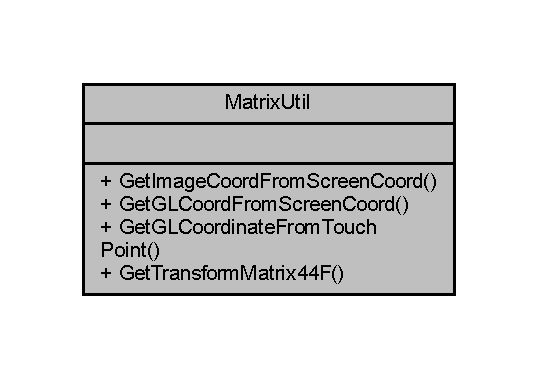
\includegraphics[width=258pt]{class_matrix_util__coll__graph}
\end{center}
\end{figure}
\subsection*{Static Public Member Functions}
\begin{DoxyCompactItemize}
\item 
static void \hyperlink{class_matrix_util_a8f1decb02c479ea6831e7baa7cf77a38}{Get\+Image\+Coord\+From\+Screen\+Coord} (int screen\+Width, int screen\+Height, int image\+Width, int image\+Height, int screenX, int screenY, int \&imageX, int \&imageY)
\item 
static void \hyperlink{class_matrix_util_a6d00d7dae3bb1c5b685adc3ea191e89e}{Get\+G\+L\+Coord\+From\+Screen\+Coord} (int screen\+Width, int screen\+Height, int image\+Width, int image\+Height, int screenX, int screenY, float \&glX, float \&glY)
\item 
static void \hyperlink{class_matrix_util_a2efb998ca1494b7c6c2887eaa4ca268f}{Get\+G\+L\+Coordinate\+From\+Touch\+Point} (int surface\+Width, int surface\+Height, int image\+Width, int image\+Height, int touchX, int touchY, float \&result\+G\+LX, float \&result\+G\+LY)
\item 
static void \hyperlink{class_matrix_util_a6a1d9aa13dc395bd7a8940ea6784b34e}{Get\+Transform\+Matrix44F} (int image\+Width, int image\+Height, gl\+\_\+helper\+::\+Mat3 input\+Transform\+Matrix33F, gl\+\_\+helper\+::\+Mat4 \&result\+Transform\+Matrix44F)
\end{DoxyCompactItemize}


\subsection{Member Function Documentation}
\mbox{\Hypertarget{class_matrix_util_a6d00d7dae3bb1c5b685adc3ea191e89e}\label{class_matrix_util_a6d00d7dae3bb1c5b685adc3ea191e89e}} 
\index{Matrix\+Util@{Matrix\+Util}!Get\+G\+L\+Coord\+From\+Screen\+Coord@{Get\+G\+L\+Coord\+From\+Screen\+Coord}}
\index{Get\+G\+L\+Coord\+From\+Screen\+Coord@{Get\+G\+L\+Coord\+From\+Screen\+Coord}!Matrix\+Util@{Matrix\+Util}}
\subsubsection{\texorpdfstring{Get\+G\+L\+Coord\+From\+Screen\+Coord()}{GetGLCoordFromScreenCoord()}}
{\footnotesize\ttfamily static void Matrix\+Util\+::\+Get\+G\+L\+Coord\+From\+Screen\+Coord (\begin{DoxyParamCaption}\item[{int}]{screen\+Width,  }\item[{int}]{screen\+Height,  }\item[{int}]{image\+Width,  }\item[{int}]{image\+Height,  }\item[{int}]{screenX,  }\item[{int}]{screenY,  }\item[{float \&}]{glX,  }\item[{float \&}]{glY }\end{DoxyParamCaption})\hspace{0.3cm}{\ttfamily [inline]}, {\ttfamily [static]}}

\mbox{\Hypertarget{class_matrix_util_a2efb998ca1494b7c6c2887eaa4ca268f}\label{class_matrix_util_a2efb998ca1494b7c6c2887eaa4ca268f}} 
\index{Matrix\+Util@{Matrix\+Util}!Get\+G\+L\+Coordinate\+From\+Touch\+Point@{Get\+G\+L\+Coordinate\+From\+Touch\+Point}}
\index{Get\+G\+L\+Coordinate\+From\+Touch\+Point@{Get\+G\+L\+Coordinate\+From\+Touch\+Point}!Matrix\+Util@{Matrix\+Util}}
\subsubsection{\texorpdfstring{Get\+G\+L\+Coordinate\+From\+Touch\+Point()}{GetGLCoordinateFromTouchPoint()}}
{\footnotesize\ttfamily static void Matrix\+Util\+::\+Get\+G\+L\+Coordinate\+From\+Touch\+Point (\begin{DoxyParamCaption}\item[{int}]{surface\+Width,  }\item[{int}]{surface\+Height,  }\item[{int}]{image\+Width,  }\item[{int}]{image\+Height,  }\item[{int}]{touchX,  }\item[{int}]{touchY,  }\item[{float \&}]{result\+G\+LX,  }\item[{float \&}]{result\+G\+LY }\end{DoxyParamCaption})\hspace{0.3cm}{\ttfamily [inline]}, {\ttfamily [static]}}

\mbox{\Hypertarget{class_matrix_util_a8f1decb02c479ea6831e7baa7cf77a38}\label{class_matrix_util_a8f1decb02c479ea6831e7baa7cf77a38}} 
\index{Matrix\+Util@{Matrix\+Util}!Get\+Image\+Coord\+From\+Screen\+Coord@{Get\+Image\+Coord\+From\+Screen\+Coord}}
\index{Get\+Image\+Coord\+From\+Screen\+Coord@{Get\+Image\+Coord\+From\+Screen\+Coord}!Matrix\+Util@{Matrix\+Util}}
\subsubsection{\texorpdfstring{Get\+Image\+Coord\+From\+Screen\+Coord()}{GetImageCoordFromScreenCoord()}}
{\footnotesize\ttfamily static void Matrix\+Util\+::\+Get\+Image\+Coord\+From\+Screen\+Coord (\begin{DoxyParamCaption}\item[{int}]{screen\+Width,  }\item[{int}]{screen\+Height,  }\item[{int}]{image\+Width,  }\item[{int}]{image\+Height,  }\item[{int}]{screenX,  }\item[{int}]{screenY,  }\item[{int \&}]{imageX,  }\item[{int \&}]{imageY }\end{DoxyParamCaption})\hspace{0.3cm}{\ttfamily [inline]}, {\ttfamily [static]}}

\mbox{\Hypertarget{class_matrix_util_a6a1d9aa13dc395bd7a8940ea6784b34e}\label{class_matrix_util_a6a1d9aa13dc395bd7a8940ea6784b34e}} 
\index{Matrix\+Util@{Matrix\+Util}!Get\+Transform\+Matrix44F@{Get\+Transform\+Matrix44F}}
\index{Get\+Transform\+Matrix44F@{Get\+Transform\+Matrix44F}!Matrix\+Util@{Matrix\+Util}}
\subsubsection{\texorpdfstring{Get\+Transform\+Matrix44\+F()}{GetTransformMatrix44F()}}
{\footnotesize\ttfamily static void Matrix\+Util\+::\+Get\+Transform\+Matrix44F (\begin{DoxyParamCaption}\item[{int}]{image\+Width,  }\item[{int}]{image\+Height,  }\item[{gl\+\_\+helper\+::\+Mat3}]{input\+Transform\+Matrix33F,  }\item[{gl\+\_\+helper\+::\+Mat4 \&}]{result\+Transform\+Matrix44F }\end{DoxyParamCaption})\hspace{0.3cm}{\ttfamily [inline]}, {\ttfamily [static]}}



The documentation for this class was generated from the following file\+:\begin{DoxyCompactItemize}
\item 
C\+:/\+Workspace/\+Vid\+Chaser/\+Vid\+Chaser/include/\hyperlink{_matrix_util_8h}{Matrix\+Util.\+h}\end{DoxyCompactItemize}

\hypertarget{class_shader_util}{}\section{Shader\+Util Class Reference}
\label{class_shader_util}\index{Shader\+Util@{Shader\+Util}}


{\ttfamily \#include $<$Shader\+Util.\+h$>$}



Collaboration diagram for Shader\+Util\+:\nopagebreak
\begin{figure}[H]
\begin{center}
\leavevmode
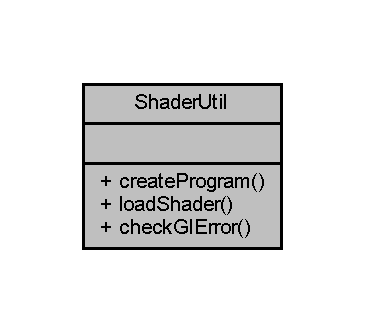
\includegraphics[width=175pt]{class_shader_util__coll__graph}
\end{center}
\end{figure}
\subsection*{Static Public Member Functions}
\begin{DoxyCompactItemize}
\item 
static unsigned int \hyperlink{class_shader_util_a1bcf8dcf6d12750db82a13321257a33e}{create\+Program} (const char $\ast$vertex\+String, const char $\ast$fragment\+String)
\item 
static unsigned int \hyperlink{class_shader_util_a5553f8c24c0182433c9bb3054035a376}{load\+Shader} (unsigned int shader\+Type, const char $\ast$p\+Source)
\item 
static void \hyperlink{class_shader_util_a3a0583a1b4016c3b30ed99a28ca2e6c9}{check\+Gl\+Error} (const char $\ast$op)
\end{DoxyCompactItemize}


\subsection{Member Function Documentation}
\mbox{\Hypertarget{class_shader_util_a3a0583a1b4016c3b30ed99a28ca2e6c9}\label{class_shader_util_a3a0583a1b4016c3b30ed99a28ca2e6c9}} 
\index{Shader\+Util@{Shader\+Util}!check\+Gl\+Error@{check\+Gl\+Error}}
\index{check\+Gl\+Error@{check\+Gl\+Error}!Shader\+Util@{Shader\+Util}}
\subsubsection{\texorpdfstring{check\+Gl\+Error()}{checkGlError()}}
{\footnotesize\ttfamily static void Shader\+Util\+::check\+Gl\+Error (\begin{DoxyParamCaption}\item[{const char $\ast$}]{op }\end{DoxyParamCaption})\hspace{0.3cm}{\ttfamily [inline]}, {\ttfamily [static]}}

Here is the caller graph for this function\+:\nopagebreak
\begin{figure}[H]
\begin{center}
\leavevmode
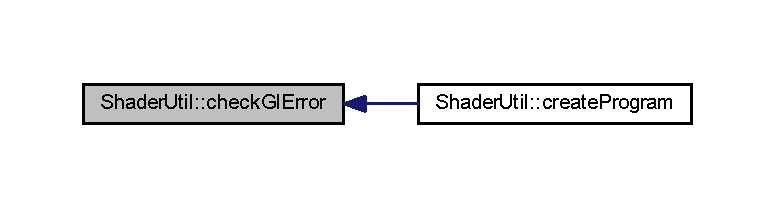
\includegraphics[width=350pt]{class_shader_util_a3a0583a1b4016c3b30ed99a28ca2e6c9_icgraph}
\end{center}
\end{figure}
\mbox{\Hypertarget{class_shader_util_a1bcf8dcf6d12750db82a13321257a33e}\label{class_shader_util_a1bcf8dcf6d12750db82a13321257a33e}} 
\index{Shader\+Util@{Shader\+Util}!create\+Program@{create\+Program}}
\index{create\+Program@{create\+Program}!Shader\+Util@{Shader\+Util}}
\subsubsection{\texorpdfstring{create\+Program()}{createProgram()}}
{\footnotesize\ttfamily static unsigned int Shader\+Util\+::create\+Program (\begin{DoxyParamCaption}\item[{const char $\ast$}]{vertex\+String,  }\item[{const char $\ast$}]{fragment\+String }\end{DoxyParamCaption})\hspace{0.3cm}{\ttfamily [inline]}, {\ttfamily [static]}}

Here is the call graph for this function\+:\nopagebreak
\begin{figure}[H]
\begin{center}
\leavevmode
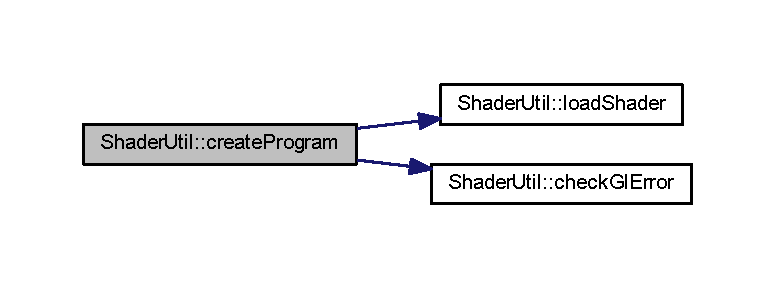
\includegraphics[width=350pt]{class_shader_util_a1bcf8dcf6d12750db82a13321257a33e_cgraph}
\end{center}
\end{figure}
\mbox{\Hypertarget{class_shader_util_a5553f8c24c0182433c9bb3054035a376}\label{class_shader_util_a5553f8c24c0182433c9bb3054035a376}} 
\index{Shader\+Util@{Shader\+Util}!load\+Shader@{load\+Shader}}
\index{load\+Shader@{load\+Shader}!Shader\+Util@{Shader\+Util}}
\subsubsection{\texorpdfstring{load\+Shader()}{loadShader()}}
{\footnotesize\ttfamily static unsigned int Shader\+Util\+::load\+Shader (\begin{DoxyParamCaption}\item[{unsigned int}]{shader\+Type,  }\item[{const char $\ast$}]{p\+Source }\end{DoxyParamCaption})\hspace{0.3cm}{\ttfamily [inline]}, {\ttfamily [static]}}

Here is the caller graph for this function\+:\nopagebreak
\begin{figure}[H]
\begin{center}
\leavevmode
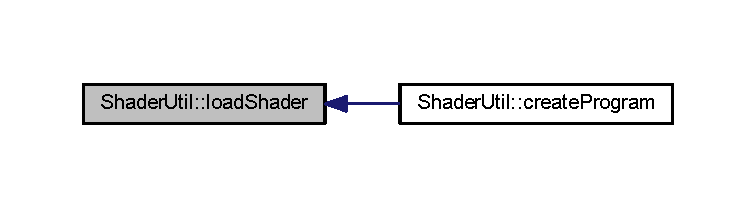
\includegraphics[width=350pt]{class_shader_util_a5553f8c24c0182433c9bb3054035a376_icgraph}
\end{center}
\end{figure}


The documentation for this class was generated from the following file\+:\begin{DoxyCompactItemize}
\item 
C\+:/\+Workspace/\+Vid\+Chaser/\+Vid\+Chaser/include/\hyperlink{_shader_util_8h}{Shader\+Util.\+h}\end{DoxyCompactItemize}

\chapter{File Documentation}
\hypertarget{_logger_8h}{}\section{C\+:/\+Workspace/\+Vid\+Chaser/\+Vid\+Chaser/include/\+Logger.h File Reference}
\label{_logger_8h}\index{C\+:/\+Workspace/\+Vid\+Chaser/\+Vid\+Chaser/include/\+Logger.\+h@{C\+:/\+Workspace/\+Vid\+Chaser/\+Vid\+Chaser/include/\+Logger.\+h}}
This graph shows which files directly or indirectly include this file\+:\nopagebreak
\begin{figure}[H]
\begin{center}
\leavevmode
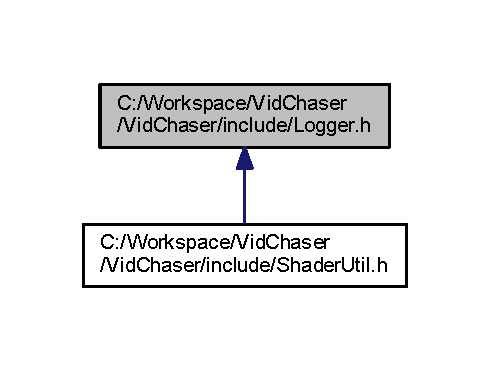
\includegraphics[width=235pt]{_logger_8h__dep__incl}
\end{center}
\end{figure}
\subsection*{Macros}
\begin{DoxyCompactItemize}
\item 
\#define \hyperlink{_logger_8h_ae9ae64d8a840f96015ae5e1421199248}{Log}(...)~printf(\+\_\+\+\_\+\+V\+A\+\_\+\+A\+R\+G\+S\+\_\+\+\_\+);
\end{DoxyCompactItemize}


\subsection{Macro Definition Documentation}
\mbox{\Hypertarget{_logger_8h_ae9ae64d8a840f96015ae5e1421199248}\label{_logger_8h_ae9ae64d8a840f96015ae5e1421199248}} 
\index{Logger.\+h@{Logger.\+h}!Log@{Log}}
\index{Log@{Log}!Logger.\+h@{Logger.\+h}}
\subsubsection{\texorpdfstring{Log}{Log}}
{\footnotesize\ttfamily \#define Log(\begin{DoxyParamCaption}\item[{}]{... }\end{DoxyParamCaption})~printf(\+\_\+\+\_\+\+V\+A\+\_\+\+A\+R\+G\+S\+\_\+\+\_\+);}


\hypertarget{_matrix_util_8h}{}\section{C\+:/\+Workspace/\+Vid\+Chaser/\+Vid\+Chaser/include/\+Matrix\+Util.h File Reference}
\label{_matrix_util_8h}\index{C\+:/\+Workspace/\+Vid\+Chaser/\+Vid\+Chaser/include/\+Matrix\+Util.\+h@{C\+:/\+Workspace/\+Vid\+Chaser/\+Vid\+Chaser/include/\+Matrix\+Util.\+h}}
{\ttfamily \#include \char`\"{}vecmath.\+h\char`\"{}}\newline
Include dependency graph for Matrix\+Util.\+h\+:\nopagebreak
\begin{figure}[H]
\begin{center}
\leavevmode
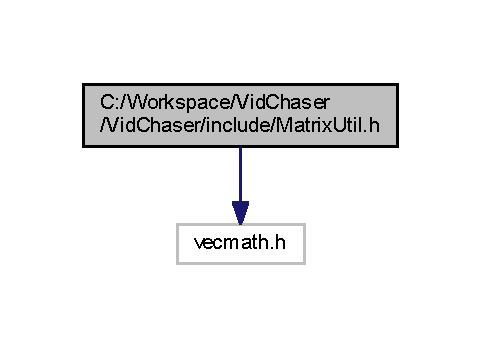
\includegraphics[width=231pt]{_matrix_util_8h__incl}
\end{center}
\end{figure}
\subsection*{Classes}
\begin{DoxyCompactItemize}
\item 
class \hyperlink{class_matrix_util}{Matrix\+Util}
\end{DoxyCompactItemize}

\hypertarget{_shader_util_8h}{}\section{C\+:/\+Workspace/\+Vid\+Chaser/\+Vid\+Chaser/include/\+Shader\+Util.h File Reference}
\label{_shader_util_8h}\index{C\+:/\+Workspace/\+Vid\+Chaser/\+Vid\+Chaser/include/\+Shader\+Util.\+h@{C\+:/\+Workspace/\+Vid\+Chaser/\+Vid\+Chaser/include/\+Shader\+Util.\+h}}
{\ttfamily \#include $<$stdlib.\+h$>$}\newline
{\ttfamily \#include $<$string$>$}\newline
{\ttfamily \#include \char`\"{}Logger.\+h\char`\"{}}\newline
Include dependency graph for Shader\+Util.\+h\+:\nopagebreak
\begin{figure}[H]
\begin{center}
\leavevmode
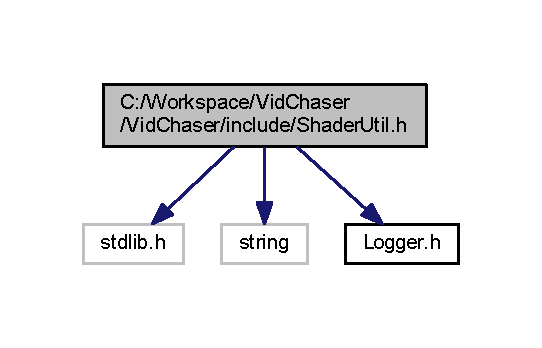
\includegraphics[width=260pt]{_shader_util_8h__incl}
\end{center}
\end{figure}
\subsection*{Classes}
\begin{DoxyCompactItemize}
\item 
class \hyperlink{class_shader_util}{Shader\+Util}
\end{DoxyCompactItemize}

\hypertarget{_vid_chaser_a_p_i_8h}{}\section{C\+:/\+Workspace/\+Vid\+Chaser/\+Vid\+Chaser/include/\+Vid\+Chaser\+A\+PI.h File Reference}
\label{_vid_chaser_a_p_i_8h}\index{C\+:/\+Workspace/\+Vid\+Chaser/\+Vid\+Chaser/include/\+Vid\+Chaser\+A\+P\+I.\+h@{C\+:/\+Workspace/\+Vid\+Chaser/\+Vid\+Chaser/include/\+Vid\+Chaser\+A\+P\+I.\+h}}
{\ttfamily \#include \char`\"{}Vid\+Chaser\+Result\+Code.\+h\char`\"{}}\newline
{\ttfamily \#include \char`\"{}Vid\+Chaser\+Define.\+h\char`\"{}}\newline
{\ttfamily \#include \char`\"{}Camera\+Preview\+Callback.\+h\char`\"{}}\newline
{\ttfamily \#include $<$string$>$}\newline
Include dependency graph for Vid\+Chaser\+A\+P\+I.\+h\+:\nopagebreak
\begin{figure}[H]
\begin{center}
\leavevmode
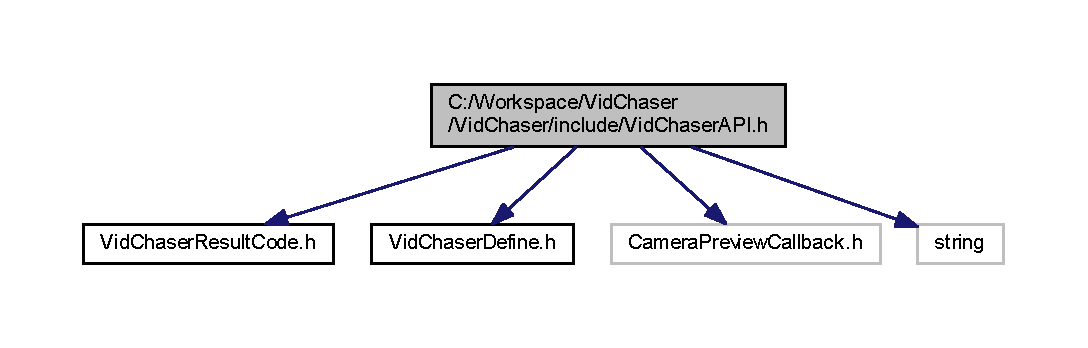
\includegraphics[width=350pt]{_vid_chaser_a_p_i_8h__incl}
\end{center}
\end{figure}
\subsection*{Namespaces}
\begin{DoxyCompactItemize}
\item 
 \hyperlink{namespace_vid_chaser}{Vid\+Chaser}
\end{DoxyCompactItemize}
\subsection*{Macros}
\begin{DoxyCompactItemize}
\item 
\#define \hyperlink{_vid_chaser_a_p_i_8h_abe868bb94e22f611aece5087695f9ef3}{V\+I\+D\+C\+H\+A\+S\+E\+R\+\_\+\+A\+PI}
\end{DoxyCompactItemize}
\subsection*{Functions}
\begin{DoxyCompactItemize}
\item 
\hyperlink{_vid_chaser_a_p_i_8h_abe868bb94e22f611aece5087695f9ef3}{V\+I\+D\+C\+H\+A\+S\+E\+R\+\_\+\+A\+PI} char $\ast$ \hyperlink{namespace_vid_chaser_a351a56150e8d7cb4a2eb78a5332f6efc}{Vid\+Chaser\+::get\+Engine\+Version} ()
\begin{DoxyCompactList}\small\item\em get engine version. \end{DoxyCompactList}\item 
\hyperlink{_vid_chaser_a_p_i_8h_abe868bb94e22f611aece5087695f9ef3}{V\+I\+D\+C\+H\+A\+S\+E\+R\+\_\+\+A\+PI} void \hyperlink{namespace_vid_chaser_a9382813c29f7bf8b97fdc9f6e2e9b51d}{Vid\+Chaser\+::start\+Camera} (int camera\+Id, int width, int height, std\+::string extra=std\+::string())
\begin{DoxyCompactList}\small\item\em start a \#camera\+Id camera with width and height resolution \end{DoxyCompactList}\item 
\hyperlink{_vid_chaser_a_p_i_8h_abe868bb94e22f611aece5087695f9ef3}{V\+I\+D\+C\+H\+A\+S\+E\+R\+\_\+\+A\+PI} void \hyperlink{namespace_vid_chaser_ad7ef05eaf00e73b7f35f760e59c5ecca}{Vid\+Chaser\+::stop\+Camera} ()
\begin{DoxyCompactList}\small\item\em close the operating camera \end{DoxyCompactList}\item 
\hyperlink{_vid_chaser_a_p_i_8h_abe868bb94e22f611aece5087695f9ef3}{V\+I\+D\+C\+H\+A\+S\+E\+R\+\_\+\+A\+PI} void \hyperlink{namespace_vid_chaser_acb17083d4c7121491e9563358d3e018f}{Vid\+Chaser\+::set\+Preview\+Callback} (Camera\+Preview\+Callback callback)
\begin{DoxyCompactList}\small\item\em register callback using camera preview buffer \end{DoxyCompactList}\item 
\hyperlink{_vid_chaser_a_p_i_8h_abe868bb94e22f611aece5087695f9ef3}{V\+I\+D\+C\+H\+A\+S\+E\+R\+\_\+\+A\+PI} void \hyperlink{namespace_vid_chaser_a563757135fd48e2a0c9b14349271c6ac}{Vid\+Chaser\+::init\+Rendering} ()
\begin{DoxyCompactList}\small\item\em initialize an internal resource for rendering \end{DoxyCompactList}\item 
\hyperlink{_vid_chaser_a_p_i_8h_abe868bb94e22f611aece5087695f9ef3}{V\+I\+D\+C\+H\+A\+S\+E\+R\+\_\+\+A\+PI} void \hyperlink{namespace_vid_chaser_afbfe1bf77862004fd5da9c95194cc506}{Vid\+Chaser\+::update\+Rendering} (int screen\+Width, int screen\+Height)
\begin{DoxyCompactList}\small\item\em input information necessary for calculating projection matrix \end{DoxyCompactList}\item 
\hyperlink{_vid_chaser_a_p_i_8h_abe868bb94e22f611aece5087695f9ef3}{V\+I\+D\+C\+H\+A\+S\+E\+R\+\_\+\+A\+PI} void \hyperlink{namespace_vid_chaser_a76a9d325e6621b9c163c5154db3f3141}{Vid\+Chaser\+::set\+Screen\+Orientation} (\hyperlink{_vid_chaser_define_8h_a5af96ebe9fdc47f01c3989cf97d41a77}{Screen\+Orientation} orientation)
\begin{DoxyCompactList}\small\item\em set Screen Orientation \end{DoxyCompactList}\item 
\hyperlink{_vid_chaser_a_p_i_8h_abe868bb94e22f611aece5087695f9ef3}{V\+I\+D\+C\+H\+A\+S\+E\+R\+\_\+\+A\+PI} void \hyperlink{namespace_vid_chaser_a68f76b454b274f9be3486792dbfd93a5}{Vid\+Chaser\+::render\+Scene} ()
\begin{DoxyCompactList}\small\item\em draw background Image. \end{DoxyCompactList}\item 
\hyperlink{_vid_chaser_a_p_i_8h_abe868bb94e22f611aece5087695f9ef3}{V\+I\+D\+C\+H\+A\+S\+E\+R\+\_\+\+A\+PI} void \hyperlink{namespace_vid_chaser_a5efdacefec8542b2d3935b87303dd442}{Vid\+Chaser\+::deinit\+Rendering} ()
\begin{DoxyCompactList}\small\item\em deinitialize an internal resource for rendering \end{DoxyCompactList}\item 
\hyperlink{_vid_chaser_a_p_i_8h_abe868bb94e22f611aece5087695f9ef3}{V\+I\+D\+C\+H\+A\+S\+E\+R\+\_\+\+A\+PI} Result\+Code \hyperlink{namespace_vid_chaser_ac6f30324b16909dc9916e2e80326ada4}{Vid\+Chaser\+::create} (std\+::string app\+Signature=\char`\"{}For\+\_\+\+Mobile\char`\"{})
\begin{DoxyCompactList}\small\item\em create Engine. \end{DoxyCompactList}\item 
\hyperlink{_vid_chaser_a_p_i_8h_abe868bb94e22f611aece5087695f9ef3}{V\+I\+D\+C\+H\+A\+S\+E\+R\+\_\+\+A\+PI} Result\+Code \hyperlink{namespace_vid_chaser_a3ef5c1fa7f048b2a32cd1d7b2dde1cd4}{Vid\+Chaser\+::add\+Tracking\+Point} (int x, int y, int $\ast$idx, \hyperlink{_vid_chaser_define_8h_ab7550d874bc06c5d36e27af27c7381e9}{Tracking\+Method} tracking\+Method=\hyperlink{_vid_chaser_define_8h_ab7550d874bc06c5d36e27af27c7381e9aecccd1296dcfe0ddcbe5954f37899f19}{Tracking\+Method\+::\+T\+R\+A\+N\+S\+L\+A\+T\+I\+ON})
\begin{DoxyCompactList}\small\item\em Add tracking position(image coordinate). \end{DoxyCompactList}\item 
\hyperlink{_vid_chaser_a_p_i_8h_abe868bb94e22f611aece5087695f9ef3}{V\+I\+D\+C\+H\+A\+S\+E\+R\+\_\+\+A\+PI} Result\+Code \hyperlink{namespace_vid_chaser_a80f0b4139cf0864085a72a5808fa6ce3}{Vid\+Chaser\+::activate\+Tracking\+Point} (int x, int y, int idx)
\begin{DoxyCompactList}\small\item\em activate tracking point \end{DoxyCompactList}\item 
\hyperlink{_vid_chaser_a_p_i_8h_abe868bb94e22f611aece5087695f9ef3}{V\+I\+D\+C\+H\+A\+S\+E\+R\+\_\+\+A\+PI} Result\+Code \hyperlink{namespace_vid_chaser_aa9d6db3ede935229cbb4322665466192}{Vid\+Chaser\+::deactivate\+Tracking\+Point} (int idx)
\begin{DoxyCompactList}\small\item\em deactivate tracking point \end{DoxyCompactList}\item 
\hyperlink{_vid_chaser_a_p_i_8h_abe868bb94e22f611aece5087695f9ef3}{V\+I\+D\+C\+H\+A\+S\+E\+R\+\_\+\+A\+PI} Result\+Code \hyperlink{namespace_vid_chaser_a3926d98471a7a7f01c2537121b27dd35}{Vid\+Chaser\+::remove\+Tracking\+Point} (int idx)
\begin{DoxyCompactList}\small\item\em Remove the tracking position of the corresponding input index. \end{DoxyCompactList}\item 
\hyperlink{_vid_chaser_a_p_i_8h_abe868bb94e22f611aece5087695f9ef3}{V\+I\+D\+C\+H\+A\+S\+E\+R\+\_\+\+A\+PI} Result\+Code \hyperlink{namespace_vid_chaser_a1ad3852918f8e289a776bbf23dde0d15}{Vid\+Chaser\+::set\+New\+Frame} (unsigned char $\ast$image, int length, int width, int height, int stride, int color\+Format, long image\+Idx)
\begin{DoxyCompactList}\small\item\em start tracking using input image. \end{DoxyCompactList}\item 
\hyperlink{_vid_chaser_a_p_i_8h_abe868bb94e22f611aece5087695f9ef3}{V\+I\+D\+C\+H\+A\+S\+E\+R\+\_\+\+A\+PI} Result\+Code \hyperlink{namespace_vid_chaser_a2174022a70838c9a9ea5c14830961a8c}{Vid\+Chaser\+::get\+Tracking\+Result} (float $\ast$transform\+Matrix3x3, int idx, int $\ast$millis)
\begin{DoxyCompactList}\small\item\em get tracking result for the index. \end{DoxyCompactList}\item 
\hyperlink{_vid_chaser_a_p_i_8h_abe868bb94e22f611aece5087695f9ef3}{V\+I\+D\+C\+H\+A\+S\+E\+R\+\_\+\+A\+PI} Result\+Code \hyperlink{namespace_vid_chaser_a1203d8bbc0f9fd8d15c8e7ad4a39d0a1}{Vid\+Chaser\+::destroy} ()
\begin{DoxyCompactList}\small\item\em destory tracking engine. \end{DoxyCompactList}\end{DoxyCompactItemize}


\subsection{Macro Definition Documentation}
\mbox{\Hypertarget{_vid_chaser_a_p_i_8h_abe868bb94e22f611aece5087695f9ef3}\label{_vid_chaser_a_p_i_8h_abe868bb94e22f611aece5087695f9ef3}} 
\index{Vid\+Chaser\+A\+P\+I.\+h@{Vid\+Chaser\+A\+P\+I.\+h}!V\+I\+D\+C\+H\+A\+S\+E\+R\+\_\+\+A\+PI@{V\+I\+D\+C\+H\+A\+S\+E\+R\+\_\+\+A\+PI}}
\index{V\+I\+D\+C\+H\+A\+S\+E\+R\+\_\+\+A\+PI@{V\+I\+D\+C\+H\+A\+S\+E\+R\+\_\+\+A\+PI}!Vid\+Chaser\+A\+P\+I.\+h@{Vid\+Chaser\+A\+P\+I.\+h}}
\subsubsection{\texorpdfstring{V\+I\+D\+C\+H\+A\+S\+E\+R\+\_\+\+A\+PI}{VIDCHASER\_API}}
{\footnotesize\ttfamily \#define V\+I\+D\+C\+H\+A\+S\+E\+R\+\_\+\+A\+PI}


\hypertarget{_vid_chaser_define_8h}{}\section{C\+:/\+Workspace/\+Vid\+Chaser/\+Vid\+Chaser/include/\+Vid\+Chaser\+Define.h File Reference}
\label{_vid_chaser_define_8h}\index{C\+:/\+Workspace/\+Vid\+Chaser/\+Vid\+Chaser/include/\+Vid\+Chaser\+Define.\+h@{C\+:/\+Workspace/\+Vid\+Chaser/\+Vid\+Chaser/include/\+Vid\+Chaser\+Define.\+h}}
This graph shows which files directly or indirectly include this file\+:\nopagebreak
\begin{figure}[H]
\begin{center}
\leavevmode
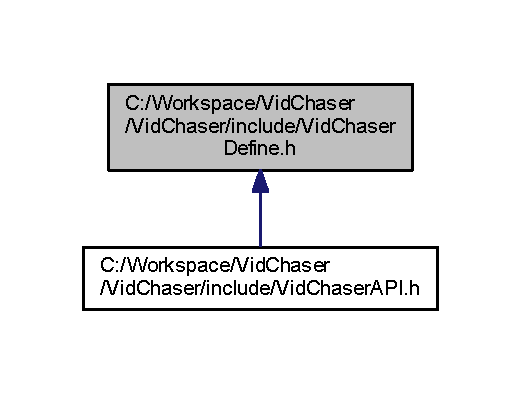
\includegraphics[width=250pt]{_vid_chaser_define_8h__dep__incl}
\end{center}
\end{figure}
\subsection*{Typedefs}
\begin{DoxyCompactItemize}
\item 
typedef unsigned char \hyperlink{_vid_chaser_define_8h_ae3a497195d617519e5353ea7b417940f}{Byte}
\end{DoxyCompactItemize}
\subsection*{Enumerations}
\begin{DoxyCompactItemize}
\item 
enum \hyperlink{_vid_chaser_define_8h_a0411236da60fe4ed141afd3f04dce8c1}{Color\+Format} \{ \newline
\hyperlink{_vid_chaser_define_8h_a0411236da60fe4ed141afd3f04dce8c1aa7c8962521c58548a2b8aed16d397d01}{R\+G\+B\+A8888} = 0, 
\hyperlink{_vid_chaser_define_8h_a0411236da60fe4ed141afd3f04dce8c1acbcf87c79628b8c7fed02f39f7cbd15f}{R\+G\+B888} = 1, 
\hyperlink{_vid_chaser_define_8h_a0411236da60fe4ed141afd3f04dce8c1aae5d89e3c7532415cd8aa46c8a7e9234}{Y\+U\+V420sp} = 2, 
\hyperlink{_vid_chaser_define_8h_a0411236da60fe4ed141afd3f04dce8c1acb52b4d8e199d901af27ee1f2d6bcb04}{Y\+U\+V420} = 3, 
\newline
\hyperlink{_vid_chaser_define_8h_a0411236da60fe4ed141afd3f04dce8c1a6ebc8e68bf90518d5bad59ab1a2dfe9f}{Y\+U\+V420\+\_\+888} = 4, 
\hyperlink{_vid_chaser_define_8h_a0411236da60fe4ed141afd3f04dce8c1ad5e2bf5600403d5c9397abc263c41ef6}{G\+R\+A\+Y8} = 5
 \}
\item 
enum \hyperlink{_vid_chaser_define_8h_ab7550d874bc06c5d36e27af27c7381e9}{Tracking\+Method} \{ \hyperlink{_vid_chaser_define_8h_ab7550d874bc06c5d36e27af27c7381e9ad9edd9e7d22a6c00c33e9024cf7511ff}{A\+F\+F\+I\+NE} = 0, 
\hyperlink{_vid_chaser_define_8h_ab7550d874bc06c5d36e27af27c7381e9a06f7b4ac3e691e7bcd5ef4a3f21bbf12}{H\+O\+M\+O\+G\+R\+A\+P\+HY} = 1, 
\hyperlink{_vid_chaser_define_8h_ab7550d874bc06c5d36e27af27c7381e9a43358c4fff77d7d5712da6d4f6d9b8e7}{R\+I\+G\+ID} = 2, 
\hyperlink{_vid_chaser_define_8h_ab7550d874bc06c5d36e27af27c7381e9aecccd1296dcfe0ddcbe5954f37899f19}{T\+R\+A\+N\+S\+L\+A\+T\+I\+ON} = 3
 \}
\item 
enum \hyperlink{_vid_chaser_define_8h_a5af96ebe9fdc47f01c3989cf97d41a77}{Screen\+Orientation} \{ \newline
\hyperlink{_vid_chaser_define_8h_a5af96ebe9fdc47f01c3989cf97d41a77a6ce26a62afab55d7606ad4e92428b30c}{U\+N\+K\+N\+O\+WN} = 0, 
\hyperlink{_vid_chaser_define_8h_a5af96ebe9fdc47f01c3989cf97d41a77af824fcbdaf7ede37030e39a2156f51e1}{P\+O\+R\+T\+R\+A\+IT} = 1, 
\hyperlink{_vid_chaser_define_8h_a5af96ebe9fdc47f01c3989cf97d41a77aeac545133a46952d1cb59892c0b8254b}{P\+O\+R\+T\+R\+A\+I\+T\+\_\+\+UP} = 1, 
\hyperlink{_vid_chaser_define_8h_a5af96ebe9fdc47f01c3989cf97d41a77af01f7caccc1e85194cb31d7e278aacc6}{P\+O\+R\+T\+R\+A\+I\+T\+\_\+\+D\+O\+WN} = 2, 
\newline
\hyperlink{_vid_chaser_define_8h_a5af96ebe9fdc47f01c3989cf97d41a77aad82a3dd15e2be2845cecf9a97017a4a}{L\+A\+N\+D\+S\+C\+A\+PE} = 3, 
\hyperlink{_vid_chaser_define_8h_a5af96ebe9fdc47f01c3989cf97d41a77a68bf2552a02c2846865d5a75dc3e170c}{L\+A\+N\+D\+S\+C\+A\+P\+E\+\_\+\+L\+E\+FT} = 3, 
\hyperlink{_vid_chaser_define_8h_a5af96ebe9fdc47f01c3989cf97d41a77ae314a57afdf2ce8311a23b9e9e6192eb}{L\+A\+N\+D\+S\+C\+A\+P\+E\+\_\+\+R\+I\+G\+HT} = 4
 \}
\end{DoxyCompactItemize}


\subsection{Typedef Documentation}
\mbox{\Hypertarget{_vid_chaser_define_8h_ae3a497195d617519e5353ea7b417940f}\label{_vid_chaser_define_8h_ae3a497195d617519e5353ea7b417940f}} 
\index{Vid\+Chaser\+Define.\+h@{Vid\+Chaser\+Define.\+h}!Byte@{Byte}}
\index{Byte@{Byte}!Vid\+Chaser\+Define.\+h@{Vid\+Chaser\+Define.\+h}}
\subsubsection{\texorpdfstring{Byte}{Byte}}
{\footnotesize\ttfamily typedef unsigned char \hyperlink{_vid_chaser_define_8h_ae3a497195d617519e5353ea7b417940f}{Byte}}



\subsection{Enumeration Type Documentation}
\mbox{\Hypertarget{_vid_chaser_define_8h_a0411236da60fe4ed141afd3f04dce8c1}\label{_vid_chaser_define_8h_a0411236da60fe4ed141afd3f04dce8c1}} 
\index{Vid\+Chaser\+Define.\+h@{Vid\+Chaser\+Define.\+h}!Color\+Format@{Color\+Format}}
\index{Color\+Format@{Color\+Format}!Vid\+Chaser\+Define.\+h@{Vid\+Chaser\+Define.\+h}}
\subsubsection{\texorpdfstring{Color\+Format}{ColorFormat}}
{\footnotesize\ttfamily enum \hyperlink{_vid_chaser_define_8h_a0411236da60fe4ed141afd3f04dce8c1}{Color\+Format}}

\begin{DoxyEnumFields}{Enumerator}
\raisebox{\heightof{T}}[0pt][0pt]{\index{R\+G\+B\+A8888@{R\+G\+B\+A8888}!Vid\+Chaser\+Define.\+h@{Vid\+Chaser\+Define.\+h}}\index{Vid\+Chaser\+Define.\+h@{Vid\+Chaser\+Define.\+h}!R\+G\+B\+A8888@{R\+G\+B\+A8888}}}\mbox{\Hypertarget{_vid_chaser_define_8h_a0411236da60fe4ed141afd3f04dce8c1aa7c8962521c58548a2b8aed16d397d01}\label{_vid_chaser_define_8h_a0411236da60fe4ed141afd3f04dce8c1aa7c8962521c58548a2b8aed16d397d01}} 
R\+G\+B\+A8888&\\
\hline

\raisebox{\heightof{T}}[0pt][0pt]{\index{R\+G\+B888@{R\+G\+B888}!Vid\+Chaser\+Define.\+h@{Vid\+Chaser\+Define.\+h}}\index{Vid\+Chaser\+Define.\+h@{Vid\+Chaser\+Define.\+h}!R\+G\+B888@{R\+G\+B888}}}\mbox{\Hypertarget{_vid_chaser_define_8h_a0411236da60fe4ed141afd3f04dce8c1acbcf87c79628b8c7fed02f39f7cbd15f}\label{_vid_chaser_define_8h_a0411236da60fe4ed141afd3f04dce8c1acbcf87c79628b8c7fed02f39f7cbd15f}} 
R\+G\+B888&\\
\hline

\raisebox{\heightof{T}}[0pt][0pt]{\index{Y\+U\+V420sp@{Y\+U\+V420sp}!Vid\+Chaser\+Define.\+h@{Vid\+Chaser\+Define.\+h}}\index{Vid\+Chaser\+Define.\+h@{Vid\+Chaser\+Define.\+h}!Y\+U\+V420sp@{Y\+U\+V420sp}}}\mbox{\Hypertarget{_vid_chaser_define_8h_a0411236da60fe4ed141afd3f04dce8c1aae5d89e3c7532415cd8aa46c8a7e9234}\label{_vid_chaser_define_8h_a0411236da60fe4ed141afd3f04dce8c1aae5d89e3c7532415cd8aa46c8a7e9234}} 
Y\+U\+V420sp&\\
\hline

\raisebox{\heightof{T}}[0pt][0pt]{\index{Y\+U\+V420@{Y\+U\+V420}!Vid\+Chaser\+Define.\+h@{Vid\+Chaser\+Define.\+h}}\index{Vid\+Chaser\+Define.\+h@{Vid\+Chaser\+Define.\+h}!Y\+U\+V420@{Y\+U\+V420}}}\mbox{\Hypertarget{_vid_chaser_define_8h_a0411236da60fe4ed141afd3f04dce8c1acb52b4d8e199d901af27ee1f2d6bcb04}\label{_vid_chaser_define_8h_a0411236da60fe4ed141afd3f04dce8c1acb52b4d8e199d901af27ee1f2d6bcb04}} 
Y\+U\+V420&\\
\hline

\raisebox{\heightof{T}}[0pt][0pt]{\index{Y\+U\+V420\+\_\+888@{Y\+U\+V420\+\_\+888}!Vid\+Chaser\+Define.\+h@{Vid\+Chaser\+Define.\+h}}\index{Vid\+Chaser\+Define.\+h@{Vid\+Chaser\+Define.\+h}!Y\+U\+V420\+\_\+888@{Y\+U\+V420\+\_\+888}}}\mbox{\Hypertarget{_vid_chaser_define_8h_a0411236da60fe4ed141afd3f04dce8c1a6ebc8e68bf90518d5bad59ab1a2dfe9f}\label{_vid_chaser_define_8h_a0411236da60fe4ed141afd3f04dce8c1a6ebc8e68bf90518d5bad59ab1a2dfe9f}} 
Y\+U\+V420\+\_\+888&\\
\hline

\raisebox{\heightof{T}}[0pt][0pt]{\index{G\+R\+A\+Y8@{G\+R\+A\+Y8}!Vid\+Chaser\+Define.\+h@{Vid\+Chaser\+Define.\+h}}\index{Vid\+Chaser\+Define.\+h@{Vid\+Chaser\+Define.\+h}!G\+R\+A\+Y8@{G\+R\+A\+Y8}}}\mbox{\Hypertarget{_vid_chaser_define_8h_a0411236da60fe4ed141afd3f04dce8c1ad5e2bf5600403d5c9397abc263c41ef6}\label{_vid_chaser_define_8h_a0411236da60fe4ed141afd3f04dce8c1ad5e2bf5600403d5c9397abc263c41ef6}} 
G\+R\+A\+Y8&\\
\hline

\end{DoxyEnumFields}
\mbox{\Hypertarget{_vid_chaser_define_8h_a5af96ebe9fdc47f01c3989cf97d41a77}\label{_vid_chaser_define_8h_a5af96ebe9fdc47f01c3989cf97d41a77}} 
\index{Vid\+Chaser\+Define.\+h@{Vid\+Chaser\+Define.\+h}!Screen\+Orientation@{Screen\+Orientation}}
\index{Screen\+Orientation@{Screen\+Orientation}!Vid\+Chaser\+Define.\+h@{Vid\+Chaser\+Define.\+h}}
\subsubsection{\texorpdfstring{Screen\+Orientation}{ScreenOrientation}}
{\footnotesize\ttfamily enum \hyperlink{_vid_chaser_define_8h_a5af96ebe9fdc47f01c3989cf97d41a77}{Screen\+Orientation}}

\begin{DoxyEnumFields}{Enumerator}
\raisebox{\heightof{T}}[0pt][0pt]{\index{U\+N\+K\+N\+O\+WN@{U\+N\+K\+N\+O\+WN}!Vid\+Chaser\+Define.\+h@{Vid\+Chaser\+Define.\+h}}\index{Vid\+Chaser\+Define.\+h@{Vid\+Chaser\+Define.\+h}!U\+N\+K\+N\+O\+WN@{U\+N\+K\+N\+O\+WN}}}\mbox{\Hypertarget{_vid_chaser_define_8h_a5af96ebe9fdc47f01c3989cf97d41a77a6ce26a62afab55d7606ad4e92428b30c}\label{_vid_chaser_define_8h_a5af96ebe9fdc47f01c3989cf97d41a77a6ce26a62afab55d7606ad4e92428b30c}} 
U\+N\+K\+N\+O\+WN&\\
\hline

\raisebox{\heightof{T}}[0pt][0pt]{\index{P\+O\+R\+T\+R\+A\+IT@{P\+O\+R\+T\+R\+A\+IT}!Vid\+Chaser\+Define.\+h@{Vid\+Chaser\+Define.\+h}}\index{Vid\+Chaser\+Define.\+h@{Vid\+Chaser\+Define.\+h}!P\+O\+R\+T\+R\+A\+IT@{P\+O\+R\+T\+R\+A\+IT}}}\mbox{\Hypertarget{_vid_chaser_define_8h_a5af96ebe9fdc47f01c3989cf97d41a77af824fcbdaf7ede37030e39a2156f51e1}\label{_vid_chaser_define_8h_a5af96ebe9fdc47f01c3989cf97d41a77af824fcbdaf7ede37030e39a2156f51e1}} 
P\+O\+R\+T\+R\+A\+IT&\\
\hline

\raisebox{\heightof{T}}[0pt][0pt]{\index{P\+O\+R\+T\+R\+A\+I\+T\+\_\+\+UP@{P\+O\+R\+T\+R\+A\+I\+T\+\_\+\+UP}!Vid\+Chaser\+Define.\+h@{Vid\+Chaser\+Define.\+h}}\index{Vid\+Chaser\+Define.\+h@{Vid\+Chaser\+Define.\+h}!P\+O\+R\+T\+R\+A\+I\+T\+\_\+\+UP@{P\+O\+R\+T\+R\+A\+I\+T\+\_\+\+UP}}}\mbox{\Hypertarget{_vid_chaser_define_8h_a5af96ebe9fdc47f01c3989cf97d41a77aeac545133a46952d1cb59892c0b8254b}\label{_vid_chaser_define_8h_a5af96ebe9fdc47f01c3989cf97d41a77aeac545133a46952d1cb59892c0b8254b}} 
P\+O\+R\+T\+R\+A\+I\+T\+\_\+\+UP&\\
\hline

\raisebox{\heightof{T}}[0pt][0pt]{\index{P\+O\+R\+T\+R\+A\+I\+T\+\_\+\+D\+O\+WN@{P\+O\+R\+T\+R\+A\+I\+T\+\_\+\+D\+O\+WN}!Vid\+Chaser\+Define.\+h@{Vid\+Chaser\+Define.\+h}}\index{Vid\+Chaser\+Define.\+h@{Vid\+Chaser\+Define.\+h}!P\+O\+R\+T\+R\+A\+I\+T\+\_\+\+D\+O\+WN@{P\+O\+R\+T\+R\+A\+I\+T\+\_\+\+D\+O\+WN}}}\mbox{\Hypertarget{_vid_chaser_define_8h_a5af96ebe9fdc47f01c3989cf97d41a77af01f7caccc1e85194cb31d7e278aacc6}\label{_vid_chaser_define_8h_a5af96ebe9fdc47f01c3989cf97d41a77af01f7caccc1e85194cb31d7e278aacc6}} 
P\+O\+R\+T\+R\+A\+I\+T\+\_\+\+D\+O\+WN&\\
\hline

\raisebox{\heightof{T}}[0pt][0pt]{\index{L\+A\+N\+D\+S\+C\+A\+PE@{L\+A\+N\+D\+S\+C\+A\+PE}!Vid\+Chaser\+Define.\+h@{Vid\+Chaser\+Define.\+h}}\index{Vid\+Chaser\+Define.\+h@{Vid\+Chaser\+Define.\+h}!L\+A\+N\+D\+S\+C\+A\+PE@{L\+A\+N\+D\+S\+C\+A\+PE}}}\mbox{\Hypertarget{_vid_chaser_define_8h_a5af96ebe9fdc47f01c3989cf97d41a77aad82a3dd15e2be2845cecf9a97017a4a}\label{_vid_chaser_define_8h_a5af96ebe9fdc47f01c3989cf97d41a77aad82a3dd15e2be2845cecf9a97017a4a}} 
L\+A\+N\+D\+S\+C\+A\+PE&\\
\hline

\raisebox{\heightof{T}}[0pt][0pt]{\index{L\+A\+N\+D\+S\+C\+A\+P\+E\+\_\+\+L\+E\+FT@{L\+A\+N\+D\+S\+C\+A\+P\+E\+\_\+\+L\+E\+FT}!Vid\+Chaser\+Define.\+h@{Vid\+Chaser\+Define.\+h}}\index{Vid\+Chaser\+Define.\+h@{Vid\+Chaser\+Define.\+h}!L\+A\+N\+D\+S\+C\+A\+P\+E\+\_\+\+L\+E\+FT@{L\+A\+N\+D\+S\+C\+A\+P\+E\+\_\+\+L\+E\+FT}}}\mbox{\Hypertarget{_vid_chaser_define_8h_a5af96ebe9fdc47f01c3989cf97d41a77a68bf2552a02c2846865d5a75dc3e170c}\label{_vid_chaser_define_8h_a5af96ebe9fdc47f01c3989cf97d41a77a68bf2552a02c2846865d5a75dc3e170c}} 
L\+A\+N\+D\+S\+C\+A\+P\+E\+\_\+\+L\+E\+FT&\\
\hline

\raisebox{\heightof{T}}[0pt][0pt]{\index{L\+A\+N\+D\+S\+C\+A\+P\+E\+\_\+\+R\+I\+G\+HT@{L\+A\+N\+D\+S\+C\+A\+P\+E\+\_\+\+R\+I\+G\+HT}!Vid\+Chaser\+Define.\+h@{Vid\+Chaser\+Define.\+h}}\index{Vid\+Chaser\+Define.\+h@{Vid\+Chaser\+Define.\+h}!L\+A\+N\+D\+S\+C\+A\+P\+E\+\_\+\+R\+I\+G\+HT@{L\+A\+N\+D\+S\+C\+A\+P\+E\+\_\+\+R\+I\+G\+HT}}}\mbox{\Hypertarget{_vid_chaser_define_8h_a5af96ebe9fdc47f01c3989cf97d41a77ae314a57afdf2ce8311a23b9e9e6192eb}\label{_vid_chaser_define_8h_a5af96ebe9fdc47f01c3989cf97d41a77ae314a57afdf2ce8311a23b9e9e6192eb}} 
L\+A\+N\+D\+S\+C\+A\+P\+E\+\_\+\+R\+I\+G\+HT&\\
\hline

\end{DoxyEnumFields}
\mbox{\Hypertarget{_vid_chaser_define_8h_ab7550d874bc06c5d36e27af27c7381e9}\label{_vid_chaser_define_8h_ab7550d874bc06c5d36e27af27c7381e9}} 
\index{Vid\+Chaser\+Define.\+h@{Vid\+Chaser\+Define.\+h}!Tracking\+Method@{Tracking\+Method}}
\index{Tracking\+Method@{Tracking\+Method}!Vid\+Chaser\+Define.\+h@{Vid\+Chaser\+Define.\+h}}
\subsubsection{\texorpdfstring{Tracking\+Method}{TrackingMethod}}
{\footnotesize\ttfamily enum \hyperlink{_vid_chaser_define_8h_ab7550d874bc06c5d36e27af27c7381e9}{Tracking\+Method}}

\begin{DoxyEnumFields}{Enumerator}
\raisebox{\heightof{T}}[0pt][0pt]{\index{A\+F\+F\+I\+NE@{A\+F\+F\+I\+NE}!Vid\+Chaser\+Define.\+h@{Vid\+Chaser\+Define.\+h}}\index{Vid\+Chaser\+Define.\+h@{Vid\+Chaser\+Define.\+h}!A\+F\+F\+I\+NE@{A\+F\+F\+I\+NE}}}\mbox{\Hypertarget{_vid_chaser_define_8h_ab7550d874bc06c5d36e27af27c7381e9ad9edd9e7d22a6c00c33e9024cf7511ff}\label{_vid_chaser_define_8h_ab7550d874bc06c5d36e27af27c7381e9ad9edd9e7d22a6c00c33e9024cf7511ff}} 
A\+F\+F\+I\+NE&\\
\hline

\raisebox{\heightof{T}}[0pt][0pt]{\index{H\+O\+M\+O\+G\+R\+A\+P\+HY@{H\+O\+M\+O\+G\+R\+A\+P\+HY}!Vid\+Chaser\+Define.\+h@{Vid\+Chaser\+Define.\+h}}\index{Vid\+Chaser\+Define.\+h@{Vid\+Chaser\+Define.\+h}!H\+O\+M\+O\+G\+R\+A\+P\+HY@{H\+O\+M\+O\+G\+R\+A\+P\+HY}}}\mbox{\Hypertarget{_vid_chaser_define_8h_ab7550d874bc06c5d36e27af27c7381e9a06f7b4ac3e691e7bcd5ef4a3f21bbf12}\label{_vid_chaser_define_8h_ab7550d874bc06c5d36e27af27c7381e9a06f7b4ac3e691e7bcd5ef4a3f21bbf12}} 
H\+O\+M\+O\+G\+R\+A\+P\+HY&\\
\hline

\raisebox{\heightof{T}}[0pt][0pt]{\index{R\+I\+G\+ID@{R\+I\+G\+ID}!Vid\+Chaser\+Define.\+h@{Vid\+Chaser\+Define.\+h}}\index{Vid\+Chaser\+Define.\+h@{Vid\+Chaser\+Define.\+h}!R\+I\+G\+ID@{R\+I\+G\+ID}}}\mbox{\Hypertarget{_vid_chaser_define_8h_ab7550d874bc06c5d36e27af27c7381e9a43358c4fff77d7d5712da6d4f6d9b8e7}\label{_vid_chaser_define_8h_ab7550d874bc06c5d36e27af27c7381e9a43358c4fff77d7d5712da6d4f6d9b8e7}} 
R\+I\+G\+ID&\\
\hline

\raisebox{\heightof{T}}[0pt][0pt]{\index{T\+R\+A\+N\+S\+L\+A\+T\+I\+ON@{T\+R\+A\+N\+S\+L\+A\+T\+I\+ON}!Vid\+Chaser\+Define.\+h@{Vid\+Chaser\+Define.\+h}}\index{Vid\+Chaser\+Define.\+h@{Vid\+Chaser\+Define.\+h}!T\+R\+A\+N\+S\+L\+A\+T\+I\+ON@{T\+R\+A\+N\+S\+L\+A\+T\+I\+ON}}}\mbox{\Hypertarget{_vid_chaser_define_8h_ab7550d874bc06c5d36e27af27c7381e9aecccd1296dcfe0ddcbe5954f37899f19}\label{_vid_chaser_define_8h_ab7550d874bc06c5d36e27af27c7381e9aecccd1296dcfe0ddcbe5954f37899f19}} 
T\+R\+A\+N\+S\+L\+A\+T\+I\+ON&\\
\hline

\end{DoxyEnumFields}

\hypertarget{_vid_chaser_result_code_8h}{}\section{C\+:/\+Workspace/\+Vid\+Chaser/\+Vid\+Chaser/include/\+Vid\+Chaser\+Result\+Code.h File Reference}
\label{_vid_chaser_result_code_8h}\index{C\+:/\+Workspace/\+Vid\+Chaser/\+Vid\+Chaser/include/\+Vid\+Chaser\+Result\+Code.\+h@{C\+:/\+Workspace/\+Vid\+Chaser/\+Vid\+Chaser/include/\+Vid\+Chaser\+Result\+Code.\+h}}
This graph shows which files directly or indirectly include this file\+:\nopagebreak
\begin{figure}[H]
\begin{center}
\leavevmode
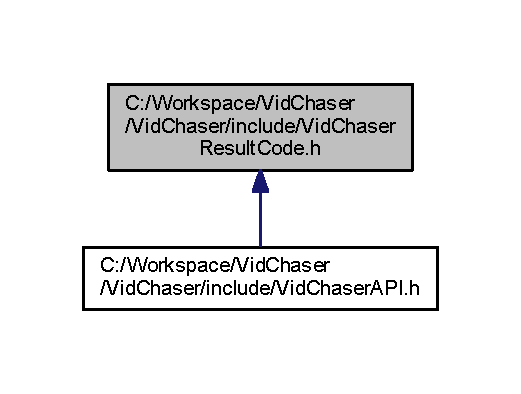
\includegraphics[width=250pt]{_vid_chaser_result_code_8h__dep__incl}
\end{center}
\end{figure}
\subsection*{Namespaces}
\begin{DoxyCompactItemize}
\item 
 \hyperlink{namespace_vid_chaser}{Vid\+Chaser}
\end{DoxyCompactItemize}
\subsection*{Enumerations}
\begin{DoxyCompactItemize}
\item 
enum \hyperlink{namespace_vid_chaser_a9a65fd4518380d53654f1af799cbf8ed}{Vid\+Chaser\+::\+Result\+Code} \{ \newline
\hyperlink{namespace_vid_chaser_a9a65fd4518380d53654f1af799cbf8eda5151e057ede3a1e7f376efbb56a0443e}{Vid\+Chaser\+::\+S\+U\+C\+C\+E\+SS} = 0, 
\hyperlink{namespace_vid_chaser_a9a65fd4518380d53654f1af799cbf8edab0d9537c24158b7ab8d23234c0808821}{Vid\+Chaser\+::\+F\+A\+IL} = 1, 
\hyperlink{namespace_vid_chaser_a9a65fd4518380d53654f1af799cbf8eda812155acd5fe876119863a7f884e7f4c}{Vid\+Chaser\+::\+M\+E\+M\+O\+R\+Y\+\_\+\+A\+L\+L\+O\+C\+A\+T\+I\+O\+N\+\_\+\+E\+R\+R\+OR} = 2, 
\hyperlink{namespace_vid_chaser_a9a65fd4518380d53654f1af799cbf8eda4d52f2f8000574e95b1ebc3dedc91298}{Vid\+Chaser\+::\+I\+N\+V\+A\+L\+I\+D\+\_\+\+A\+PP} = 10, 
\newline
\hyperlink{namespace_vid_chaser_a9a65fd4518380d53654f1af799cbf8edafd918f3fa6f9e5df38c8b0970dc0e51d}{Vid\+Chaser\+::\+T\+R\+A\+C\+K\+A\+B\+L\+E\+\_\+\+A\+L\+R\+E\+A\+D\+Y\+\_\+\+E\+X\+I\+ST} = 50, 
\hyperlink{namespace_vid_chaser_a9a65fd4518380d53654f1af799cbf8eda75a688e24ca224d5b9fe2859ea579f9c}{Vid\+Chaser\+::\+T\+R\+A\+C\+K\+A\+B\+L\+E\+\_\+\+I\+S\+\_\+\+N\+O\+T\+\_\+\+E\+X\+I\+ST} = 51, 
\hyperlink{namespace_vid_chaser_a9a65fd4518380d53654f1af799cbf8edafb2e81caca6ee6d10e83fb4a28921e39}{Vid\+Chaser\+::\+T\+R\+A\+C\+K\+A\+B\+L\+E\+\_\+\+A\+L\+R\+E\+A\+D\+Y\+\_\+\+A\+C\+T\+I\+V\+A\+T\+ED} = 52, 
\hyperlink{namespace_vid_chaser_a9a65fd4518380d53654f1af799cbf8eda2e2c5512767b66864b4db78ca8ab96ee}{Vid\+Chaser\+::\+T\+R\+A\+C\+K\+A\+B\+L\+E\+\_\+\+A\+L\+R\+E\+A\+D\+Y\+\_\+\+D\+E\+A\+C\+T\+I\+V\+A\+T\+ED} = 53, 
\newline
\hyperlink{namespace_vid_chaser_a9a65fd4518380d53654f1af799cbf8edac4e8d2fb08c509ce905b7821d8a028f1}{Vid\+Chaser\+::\+P\+I\+X\+E\+L\+\_\+\+F\+O\+R\+M\+A\+T\+\_\+\+E\+R\+R\+OR} = 60, 
\hyperlink{namespace_vid_chaser_a9a65fd4518380d53654f1af799cbf8edae75f339feb7a945186fcb40fc53280de}{Vid\+Chaser\+::\+I\+N\+P\+U\+T\+\_\+\+I\+M\+A\+G\+E\+\_\+\+E\+M\+P\+TY} = 61, 
\hyperlink{namespace_vid_chaser_a9a65fd4518380d53654f1af799cbf8eda40bd178f65d935a585199e4d178ebfe8}{Vid\+Chaser\+::\+I\+N\+P\+U\+T\+\_\+\+I\+M\+A\+G\+E\+\_\+\+R\+E\+S\+O\+L\+U\+T\+I\+O\+N\+\_\+\+E\+R\+R\+OR} = 62, 
\hyperlink{namespace_vid_chaser_a9a65fd4518380d53654f1af799cbf8edaf3c881f67a4378bb3039de82238456a5}{Vid\+Chaser\+::\+E\+N\+G\+I\+N\+E\+\_\+\+A\+L\+R\+E\+A\+D\+Y\+\_\+\+I\+N\+I\+T\+I\+A\+L\+I\+Z\+ED} = 170, 
\newline
\hyperlink{namespace_vid_chaser_a9a65fd4518380d53654f1af799cbf8edae356f1e1773cea2be2c7923c81c50b4d}{Vid\+Chaser\+::\+E\+N\+G\+I\+N\+E\+\_\+\+I\+S\+\_\+\+N\+O\+T\+\_\+\+I\+N\+I\+T\+I\+A\+L\+I\+Z\+ED} = 180, 
\hyperlink{namespace_vid_chaser_a9a65fd4518380d53654f1af799cbf8edae0af694ebbabbe2f9050b879bbab1650}{Vid\+Chaser\+::\+C\+H\+E\+C\+K\+\_\+\+L\+E\+A\+R\+N\+A\+B\+L\+E\+\_\+\+P\+I\+X\+E\+L\+F\+O\+R\+M\+A\+T\+\_\+\+E\+R\+R\+OR} = 190, 
\hyperlink{namespace_vid_chaser_a9a65fd4518380d53654f1af799cbf8edaf019ce4b932c9d8e30fcd49359e3bf2c}{Vid\+Chaser\+::\+L\+E\+A\+R\+N\+\_\+\+S\+T\+R\+O\+K\+E\+\_\+\+E\+M\+P\+TY} = 200, 
\hyperlink{namespace_vid_chaser_a9a65fd4518380d53654f1af799cbf8eda01e3cca957ead1e93450e8dbd49dc3b5}{Vid\+Chaser\+::\+L\+E\+A\+R\+N\+\_\+\+S\+T\+R\+O\+K\+E\+\_\+\+O\+V\+E\+R\+F\+L\+OW} = 201, 
\newline
\hyperlink{namespace_vid_chaser_a9a65fd4518380d53654f1af799cbf8eda3c8a1d9afcff42b2226ef6398019968d}{Vid\+Chaser\+::\+T\+R\+A\+C\+K\+E\+R\+\_\+\+A\+L\+R\+E\+A\+D\+Y\+\_\+\+S\+T\+A\+R\+T\+ED} = 300, 
\hyperlink{namespace_vid_chaser_a9a65fd4518380d53654f1af799cbf8eda0f6a6c38af8fed9e2315c7ca598470c9}{Vid\+Chaser\+::\+T\+R\+A\+C\+K\+E\+R\+\_\+\+A\+L\+R\+E\+A\+D\+Y\+\_\+\+S\+T\+O\+P\+ED} = 310, 
\hyperlink{namespace_vid_chaser_a9a65fd4518380d53654f1af799cbf8eda5c335d57b3c769c7eb00213f69d13b0b}{Vid\+Chaser\+::\+I\+N\+P\+U\+T\+\_\+\+T\+R\+A\+C\+K\+A\+B\+L\+E\+\_\+\+E\+M\+P\+TY} = 320, 
\hyperlink{namespace_vid_chaser_a9a65fd4518380d53654f1af799cbf8eda1099645fafffff33a4e4db2aab5abb4d}{Vid\+Chaser\+::\+U\+N\+D\+E\+F\+I\+N\+E\+\_\+\+E\+R\+R\+OR} = 99
 \}
\end{DoxyCompactItemize}

%--- End generated contents ---

% Index
\backmatter
\newpage
\phantomsection
\clearemptydoublepage
\addcontentsline{toc}{chapter}{Index}
\printindex

\end{document}
